% Options for packages loaded elsewhere
\PassOptionsToPackage{unicode}{hyperref}
\PassOptionsToPackage{hyphens}{url}
\PassOptionsToPackage{dvipsnames,svgnames,x11names}{xcolor}
%
\documentclass[
  letterpaper,
]{krantz}

\usepackage{amsmath,amssymb}
\usepackage{iftex}
\ifPDFTeX
  \usepackage[T1]{fontenc}
  \usepackage[utf8]{inputenc}
  \usepackage{textcomp} % provide euro and other symbols
\else % if luatex or xetex
  \usepackage{unicode-math}
  \defaultfontfeatures{Scale=MatchLowercase}
  \defaultfontfeatures[\rmfamily]{Ligatures=TeX,Scale=1}
\fi
\usepackage{lmodern}
\ifPDFTeX\else  
    % xetex/luatex font selection
\fi
% Use upquote if available, for straight quotes in verbatim environments
\IfFileExists{upquote.sty}{\usepackage{upquote}}{}
\IfFileExists{microtype.sty}{% use microtype if available
  \usepackage[]{microtype}
  \UseMicrotypeSet[protrusion]{basicmath} % disable protrusion for tt fonts
}{}
\makeatletter
\@ifundefined{KOMAClassName}{% if non-KOMA class
  \IfFileExists{parskip.sty}{%
    \usepackage{parskip}
  }{% else
    \setlength{\parindent}{0pt}
    \setlength{\parskip}{6pt plus 2pt minus 1pt}}
}{% if KOMA class
  \KOMAoptions{parskip=half}}
\makeatother
\usepackage{xcolor}
\setlength{\emergencystretch}{3em} % prevent overfull lines
\setcounter{secnumdepth}{5}
% Make \paragraph and \subparagraph free-standing
\ifx\paragraph\undefined\else
  \let\oldparagraph\paragraph
  \renewcommand{\paragraph}[1]{\oldparagraph{#1}\mbox{}}
\fi
\ifx\subparagraph\undefined\else
  \let\oldsubparagraph\subparagraph
  \renewcommand{\subparagraph}[1]{\oldsubparagraph{#1}\mbox{}}
\fi

\usepackage{color}
\usepackage{fancyvrb}
\newcommand{\VerbBar}{|}
\newcommand{\VERB}{\Verb[commandchars=\\\{\}]}
\DefineVerbatimEnvironment{Highlighting}{Verbatim}{commandchars=\\\{\}}
% Add ',fontsize=\small' for more characters per line
\usepackage{framed}
\definecolor{shadecolor}{RGB}{241,243,245}
\newenvironment{Shaded}{\begin{snugshade}}{\end{snugshade}}
\newcommand{\AlertTok}[1]{\textcolor[rgb]{0.68,0.00,0.00}{#1}}
\newcommand{\AnnotationTok}[1]{\textcolor[rgb]{0.37,0.37,0.37}{#1}}
\newcommand{\AttributeTok}[1]{\textcolor[rgb]{0.40,0.45,0.13}{#1}}
\newcommand{\BaseNTok}[1]{\textcolor[rgb]{0.68,0.00,0.00}{#1}}
\newcommand{\BuiltInTok}[1]{\textcolor[rgb]{0.00,0.23,0.31}{#1}}
\newcommand{\CharTok}[1]{\textcolor[rgb]{0.13,0.47,0.30}{#1}}
\newcommand{\CommentTok}[1]{\textcolor[rgb]{0.37,0.37,0.37}{#1}}
\newcommand{\CommentVarTok}[1]{\textcolor[rgb]{0.37,0.37,0.37}{\textit{#1}}}
\newcommand{\ConstantTok}[1]{\textcolor[rgb]{0.56,0.35,0.01}{#1}}
\newcommand{\ControlFlowTok}[1]{\textcolor[rgb]{0.00,0.23,0.31}{#1}}
\newcommand{\DataTypeTok}[1]{\textcolor[rgb]{0.68,0.00,0.00}{#1}}
\newcommand{\DecValTok}[1]{\textcolor[rgb]{0.68,0.00,0.00}{#1}}
\newcommand{\DocumentationTok}[1]{\textcolor[rgb]{0.37,0.37,0.37}{\textit{#1}}}
\newcommand{\ErrorTok}[1]{\textcolor[rgb]{0.68,0.00,0.00}{#1}}
\newcommand{\ExtensionTok}[1]{\textcolor[rgb]{0.00,0.23,0.31}{#1}}
\newcommand{\FloatTok}[1]{\textcolor[rgb]{0.68,0.00,0.00}{#1}}
\newcommand{\FunctionTok}[1]{\textcolor[rgb]{0.28,0.35,0.67}{#1}}
\newcommand{\ImportTok}[1]{\textcolor[rgb]{0.00,0.46,0.62}{#1}}
\newcommand{\InformationTok}[1]{\textcolor[rgb]{0.37,0.37,0.37}{#1}}
\newcommand{\KeywordTok}[1]{\textcolor[rgb]{0.00,0.23,0.31}{#1}}
\newcommand{\NormalTok}[1]{\textcolor[rgb]{0.00,0.23,0.31}{#1}}
\newcommand{\OperatorTok}[1]{\textcolor[rgb]{0.37,0.37,0.37}{#1}}
\newcommand{\OtherTok}[1]{\textcolor[rgb]{0.00,0.23,0.31}{#1}}
\newcommand{\PreprocessorTok}[1]{\textcolor[rgb]{0.68,0.00,0.00}{#1}}
\newcommand{\RegionMarkerTok}[1]{\textcolor[rgb]{0.00,0.23,0.31}{#1}}
\newcommand{\SpecialCharTok}[1]{\textcolor[rgb]{0.37,0.37,0.37}{#1}}
\newcommand{\SpecialStringTok}[1]{\textcolor[rgb]{0.13,0.47,0.30}{#1}}
\newcommand{\StringTok}[1]{\textcolor[rgb]{0.13,0.47,0.30}{#1}}
\newcommand{\VariableTok}[1]{\textcolor[rgb]{0.07,0.07,0.07}{#1}}
\newcommand{\VerbatimStringTok}[1]{\textcolor[rgb]{0.13,0.47,0.30}{#1}}
\newcommand{\WarningTok}[1]{\textcolor[rgb]{0.37,0.37,0.37}{\textit{#1}}}

\providecommand{\tightlist}{%
  \setlength{\itemsep}{0pt}\setlength{\parskip}{0pt}}\usepackage{longtable,booktabs,array}
\usepackage{calc} % for calculating minipage widths
% Correct order of tables after \paragraph or \subparagraph
\usepackage{etoolbox}
\makeatletter
\patchcmd\longtable{\par}{\if@noskipsec\mbox{}\fi\par}{}{}
\makeatother
% Allow footnotes in longtable head/foot
\IfFileExists{footnotehyper.sty}{\usepackage{footnotehyper}}{\usepackage{footnote}}
\makesavenoteenv{longtable}
\usepackage{graphicx}
\makeatletter
\def\maxwidth{\ifdim\Gin@nat@width>\linewidth\linewidth\else\Gin@nat@width\fi}
\def\maxheight{\ifdim\Gin@nat@height>\textheight\textheight\else\Gin@nat@height\fi}
\makeatother
% Scale images if necessary, so that they will not overflow the page
% margins by default, and it is still possible to overwrite the defaults
% using explicit options in \includegraphics[width, height, ...]{}
\setkeys{Gin}{width=\maxwidth,height=\maxheight,keepaspectratio}
% Set default figure placement to htbp
\makeatletter
\def\fps@figure{htbp}
\makeatother
\newlength{\cslhangindent}
\setlength{\cslhangindent}{1.5em}
\newlength{\csllabelwidth}
\setlength{\csllabelwidth}{3em}
\newlength{\cslentryspacingunit} % times entry-spacing
\setlength{\cslentryspacingunit}{\parskip}
\newenvironment{CSLReferences}[2] % #1 hanging-ident, #2 entry spacing
 {% don't indent paragraphs
  \setlength{\parindent}{0pt}
  % turn on hanging indent if param 1 is 1
  \ifodd #1
  \let\oldpar\par
  \def\par{\hangindent=\cslhangindent\oldpar}
  \fi
  % set entry spacing
  \setlength{\parskip}{#2\cslentryspacingunit}
 }%
 {}
\usepackage{calc}
\newcommand{\CSLBlock}[1]{#1\hfill\break}
\newcommand{\CSLLeftMargin}[1]{\parbox[t]{\csllabelwidth}{#1}}
\newcommand{\CSLRightInline}[1]{\parbox[t]{\linewidth - \csllabelwidth}{#1}\break}
\newcommand{\CSLIndent}[1]{\hspace{\cslhangindent}#1}

\usepackage{booktabs}
\usepackage{longtable}
\usepackage[bf,singlelinecheck=off]{caption}
\usepackage[scale=.8]{sourcecodepro}
\usepackage{hyperref}

\usepackage{framed,color}
\definecolor{shadecolor}{RGB}{248,248,248}

\renewcommand{\textfraction}{0.05}
\renewcommand{\topfraction}{0.8}
\renewcommand{\bottomfraction}{0.8}
\renewcommand{\floatpagefraction}{0.75}

\renewenvironment{quote}{\begin{VF}}{\end{VF}}
\let\oldhref\href
\renewcommand{\href}[2]{#2\footnote{\url{#1}}}

\makeatletter
\newenvironment{kframe}{%
\medskip{}
\setlength{\fboxsep}{.8em}
 \def\at@end@of@kframe{}%
 \ifinner\ifhmode%
  \def\at@end@of@kframe{\end{minipage}}%
  \begin{minipage}{\columnwidth}%
 \fi\fi%
 \def\FrameCommand##1{\hskip\@totalleftmargin \hskip-\fboxsep
 \colorbox{shadecolor}{##1}\hskip-\fboxsep
     % There is no \\@totalrightmargin, so:
     \hskip-\linewidth \hskip-\@totalleftmargin \hskip\columnwidth}%
 \MakeFramed {\advance\hsize-\width
   \@totalleftmargin\z@ \linewidth\hsize
   \@setminipage}}%
 {\par\unskip\endMakeFramed%
 \at@end@of@kframe}
\makeatother

\renewenvironment{Shaded}{\begin{kframe}}{\end{kframe}}

\usepackage{makeidx}
\makeindex

\urlstyle{tt}

\usepackage{amsthm}
\makeatletter
\def\thm@space@setup{%
  \thm@preskip=8pt plus 2pt minus 4pt
  \thm@postskip=\thm@preskip
}
\makeatother

\frontmatter
\makeatletter
\makeatother
\makeatletter
\@ifpackageloaded{bookmark}{}{\usepackage{bookmark}}
\makeatother
\makeatletter
\@ifpackageloaded{caption}{}{\usepackage{caption}}
\AtBeginDocument{%
\ifdefined\contentsname
  \renewcommand*\contentsname{Table of contents}
\else
  \newcommand\contentsname{Table of contents}
\fi
\ifdefined\listfigurename
  \renewcommand*\listfigurename{List of Figures}
\else
  \newcommand\listfigurename{List of Figures}
\fi
\ifdefined\listtablename
  \renewcommand*\listtablename{List of Tables}
\else
  \newcommand\listtablename{List of Tables}
\fi
\ifdefined\figurename
  \renewcommand*\figurename{Figure}
\else
  \newcommand\figurename{Figure}
\fi
\ifdefined\tablename
  \renewcommand*\tablename{Table}
\else
  \newcommand\tablename{Table}
\fi
}
\@ifpackageloaded{float}{}{\usepackage{float}}
\floatstyle{ruled}
\@ifundefined{c@chapter}{\newfloat{codelisting}{h}{lop}}{\newfloat{codelisting}{h}{lop}[chapter]}
\floatname{codelisting}{Listing}
\newcommand*\listoflistings{\listof{codelisting}{List of Listings}}
\makeatother
\makeatletter
\@ifpackageloaded{caption}{}{\usepackage{caption}}
\@ifpackageloaded{subcaption}{}{\usepackage{subcaption}}
\makeatother
\makeatletter
\@ifpackageloaded{tcolorbox}{}{\usepackage[skins,breakable]{tcolorbox}}
\makeatother
\makeatletter
\@ifundefined{shadecolor}{\definecolor{shadecolor}{rgb}{.97, .97, .97}}
\makeatother
\makeatletter
\makeatother
\makeatletter
\makeatother
\ifLuaTeX
  \usepackage{selnolig}  % disable illegal ligatures
\fi
\IfFileExists{bookmark.sty}{\usepackage{bookmark}}{\usepackage{hyperref}}
\IfFileExists{xurl.sty}{\usepackage{xurl}}{} % add URL line breaks if available
\urlstyle{same} % disable monospaced font for URLs
\hypersetup{
  pdftitle={Quarto CRC Book},
  pdfauthor={Jane Doe and Max Power},
  colorlinks=true,
  linkcolor={blue},
  filecolor={Maroon},
  citecolor={Blue},
  urlcolor={Blue},
  pdfcreator={LaTeX via pandoc}}

\title{Quarto CRC Book}
\author{Jane Doe and Max Power}
\date{2022-11-22}

\begin{document}
\maketitle
% you may need to leave a few empty pages before the dedication page

%\cleardoublepage\newpage\thispagestyle{empty}\null
%\cleardoublepage\newpage\thispagestyle{empty}\null
%\cleardoublepage\newpage
\thispagestyle{empty}

\begin{center}
To blah, blah, and blah.
%\includegraphics{images/dedication.pdf}
\end{center}

\setlength{\abovedisplayskip}{-5pt}
\setlength{\abovedisplayshortskip}{-5pt}

\ifdefined\Shaded\renewenvironment{Shaded}{\begin{tcolorbox}[frame hidden, interior hidden, breakable, boxrule=0pt, borderline west={3pt}{0pt}{shadecolor}, sharp corners, enhanced]}{\end{tcolorbox}}\fi

\renewcommand*\contentsname{Table of contents}
{
\hypersetup{linkcolor=}
\setcounter{tocdepth}{2}
\tableofcontents
}
\bookmarksetup{startatroot}

\hypertarget{proyek-sains-data}{%
\chapter*{Proyek Sains data}\label{proyek-sains-data}}
\addcontentsline{toc}{chapter}{Proyek Sains data}

\markboth{Proyek Sains data}{Proyek Sains data}

Nama : Sadam payoda sabilillah

NIM : 200411100069

\bookmarksetup{startatroot}

\hypertarget{bussines-understanding}{%
\chapter*{bussines Understanding}\label{bussines-understanding}}
\addcontentsline{toc}{chapter}{bussines Understanding}

\markboth{bussines Understanding}{bussines Understanding}

Tujuannya apa untuk mengumpulkan data tersebut dan kenapa kita harus
mengumpulkan data Cirrhosis Patient Survival Prediction :

\begin{enumerate}
\def\labelenumi{\arabic{enumi}.}
\item
  Melalui analisis data, peneliti ilmiah dapat mengidentifikasi
  faktor-faktor risiko apa saja yang berkaitan dengan kelangsungan hidup
  pasien. Ini dapat mencakup faktor-faktor seperti tingkat keparahan
  sirosis, komplikasi lainnya, dan respons terhadap pengobatan.
\item
  menganalisis data untuk membantu djaalam memahami efektivitas berbagai
  jenis perawatan dan intervensi pada pasien dengan sirosis hati. Hal
  ini dapat membantu dokter dalam merencanakan perawatan yang lebih
  efektif dan tepat waktu agar kemungkinan pada kehidupan penderita
  sironis hati menjadi lebih aman atau akurasi keberlangsungan hiduo
  menjadi panjang.
\item
  dengan adanya Informasi dataset Cirrhosis Patient Survival Prediction
  dengan pengidap prognosis sirosis hati dapat digunakan untuk
  memberikan edukasi kepada masyarakat tentang faktor risiko dan
  pentingnya deteksi dini. Kesadaran ini dapat meningkatkan upaya
  pencegahan dan deteksi dini kondisi yang dapat menyebabkan sirosis
  hati.
\end{enumerate}

Diatas adalah beberapa tujuan pentingnya untuk mengumpulkan data data
CDC Diabetes Health Indicator.

\bookmarksetup{startatroot}

\hypertarget{data-understanding}{%
\chapter*{Data Understanding}\label{data-understanding}}
\addcontentsline{toc}{chapter}{Data Understanding}

\markboth{Data Understanding}{Data Understanding}

\hypertarget{cirrhosis-patient-survival-prediction}{%
\section*{Cirrhosis Patient Survival
Prediction}\label{cirrhosis-patient-survival-prediction}}
\addcontentsline{toc}{section}{Cirrhosis Patient Survival Prediction}

\markright{Cirrhosis Patient Survival Prediction}

\textbf{Cirrhosis Patient Survival Prediction} seperti melakukan
prediksi kelangsungan hidup pasien yang menderita dengan penyakit
sirosis hati. Sirosis hati adalah kondisi medis yang terjadi ketika
jaringan hati normal digantikan oleh jaringan parut, yang dapat
mempengaruhi fungsi hati secara signifikan. Proses terbentuknya parut di
hati, atau sirosis hati, terjadi sebagai respons terhadap kerusakan yang
berulang pada sel hati.

\begin{itemize}
\tightlist
\item
  Untuk tujuan apa kumpulan data tersebut dibuat?
\end{itemize}

Sirosis terjadi akibat kerusakan hati yang berkepanjangan, sehingga
menimbulkan jaringan parut yang luas, sering kali disebabkan oleh
kondisi seperti hepatitis atau konsumsi alkohol kronis. Data yang
diberikan bersumber dari penelitian Mayo Clinic tentang sirosis bilier
primer (PBC) hati yang dilakukan pada tahun 1974 hingga 1984.

\hypertarget{mengenai-dataset-pada-cirrhosis-patient-survival-prediction}{%
\subsection*{Mengenai dataset pada Cirrhosis Patient Survival
Prediction}\label{mengenai-dataset-pada-cirrhosis-patient-survival-prediction}}
\addcontentsline{toc}{subsection}{Mengenai dataset pada Cirrhosis
Patient Survival Prediction}

\begin{longtable}[]{@{}
  >{\raggedright\arraybackslash}p{(\columnwidth - 2\tabcolsep) * \real{0.1404}}
  >{\raggedright\arraybackslash}p{(\columnwidth - 2\tabcolsep) * \real{0.8596}}@{}}
\toprule\noalign{}
\begin{minipage}[b]{\linewidth}\raggedright
Fitur
\end{minipage} & \begin{minipage}[b]{\linewidth}\raggedright
Penjelasan
\end{minipage} \\
\midrule\noalign{}
\endhead
\bottomrule\noalign{}
\endlastfoot
ID & Nomor identifikasi unik untuk setiap pasien. \\
N\_Days & Jumlah hari antara pendaftaran dan peristiwa akhir (kematian,
transplantasi hati, atau waktu analisis studi pada Juli 1986). \\
Status & Status pasien pada akhir periode pengamatan. Nilai melibatkan C
(censored), CL (censored karena transplantasi hati), atau D
(kematian). \\
Drug & Jenis obat yang diberikan kepada pasien (D-penicillamine atau
plasebo). \\
Age & Umur pasien pada saat pengamatan awal. \\
Sex & Jenis kelamin pasien (M atau F). \\
Ascites & Indikator keberadaan atau tingkat keparahan ascites
(penumpukan cairan di rongga perut) Ascites adalah suatu kondisi di mana
cairan berlebihan menumpuk dalam rongga perut, antara lapisan organ
dalam rongga perut (seperti hati dan usus) dan dinding perut. \\
Hepatomegaly & Hepatomegaly adalah istilah medis yang digunakan untuk
menggambarkan pembesaran hati. Hati yang sehat memiliki ukuran tertentu,
tetapi berbagai kondisi dapat menyebabkan hati menjadi lebih besar dari
ukuran normal, Indikator keberadaan atau tingkat hepatomegali
(pembesaran hati). \\
Spiders & ``SPIDERS'' yang merupakan singkatan dari ``Cirrhosis SPiders
of the Liver.'' Sistem ini dirancang untuk memberikan perkiraan risiko
kelangsungan hidup pasien dengan sirosis hati berdasarkan sejumlah
parameter klinis dan laboratorium. Indikator keberadaan atau tingkat
keparahan spider nevi (pembuluh darah kecil pada kulit, mungkin menjadi
tanda sirosis hati). \\
Edema & Edema adalah suatu kondisi medis yang ditandai oleh penumpukan
cairan yang berlebihan di dalam jaringan tubuh, biasanya di ruang
interstisial antara sel-sel. Ini dapat menyebabkan pembengkakan atau
pembesaran area yang terkena. Indikator keberadaan atau tingkat edema,
dengan nilai N (tidak ada edema dan tanpa terapi diuretik), S (edema
hadir tanpa diuretik, atau edema yang teratasi oleh diuretik), atau Y
(edema meskipun terapi diuretik). \\
Bilirubin & Kadar serum bilirubin dalam mg/dl, indikator kerusakan
hati. \\
Cholesterol & Kadar serum kolesterol dalam mg/dl. \\
Albumin & Kadar albumin dalam gm/dl, protein yang diproduksi oleh
hati. \\
Copper & Kadar tembaga dalam urine (µg/day), indikator gangguan
metabolisme tembaga. \\
Alk\_Phos & Kadar fosfatase alkali dalam U/liter, indikator kerusakan
hati atau masalah tulang. \\
SGOT & Tes darah SGOT sering dilakukan sebagai bagian dari panel fungsi
hati untuk mengevaluasi kesehatan hati dan organ-organ lain yang dapat
mengandung enzim ini. Kadar serum glutamat oksalat transaminase (SGOT)
dalam U/ml, indikator kerusakan hati. \\
Tryglicerides & Kadar trigliserida, indikator kesehatan metabolik. \\
Platelets & Jumlah trombosit per ml/1000, gangguan jumlah trombosit
terkait dengan kerusakan hati. \\
Prothrombin & Prothrombin adalah sebuah protein yang terlibat dalam
proses pembekuan darah. Ini adalah salah satu faktor pembekuan darah
yang penting dan berperan dalam mengubah fibrinogen menjadi fibrin,
suatu langkah kunci dalam pembentukan bekuan darah. Waktu protrombin
dalam detik, indikator fungsi pembekuan darah. \\
Stage & Tahap atau tingkat keparahan sirosis hati pada saat pengamatan
awal (1, 2, 3, atau 4) semakin mendekati 4 maka semakin parah. \\
\end{longtable}

\hypertarget{melakukan-pengambilan-dataset}{%
\section*{Melakukan pengambilan
dataset}\label{melakukan-pengambilan-dataset}}
\addcontentsline{toc}{section}{Melakukan pengambilan dataset}

\markright{Melakukan pengambilan dataset}

\begin{Shaded}
\begin{Highlighting}[]
\ImportTok{import}\NormalTok{ pandas }\ImportTok{as}\NormalTok{ pd}

\NormalTok{url }\OperatorTok{=} \StringTok{"cirrhosis.csv"}

\CommentTok{\# Mengimpor data ke dalam pandas DataFrame}
\NormalTok{df }\OperatorTok{=}\NormalTok{ pd.read\_csv(url)}

\NormalTok{df}
\end{Highlighting}
\end{Shaded}

\begin{longtable}[]{@{}lllllllllllllllllllll@{}}
\toprule\noalign{}
& ID & N\_Days & Status & Drug & Age & Sex & Ascites & Hepatomegaly &
Spiders & Edema & Bilirubin & Cholesterol & Albumin & Copper & Alk\_Phos
& SGOT & Tryglicerides & Platelets & Prothrombin & Stage \\
\midrule\noalign{}
\endhead
\bottomrule\noalign{}
\endlastfoot
0 & 1 & 400 & D & D-penicillamine & 21464 & F & Y & Y & Y & Y & 14.5 &
261.0 & 2.60 & 156.0 & 1718.0 & 137.95 & 172.0 & 190.0 & 12.2 & 4.0 \\
1 & 2 & 4500 & C & D-penicillamine & 20617 & F & N & Y & Y & N & 1.1 &
302.0 & 4.14 & 54.0 & 7394.8 & 113.52 & 88.0 & 221.0 & 10.6 & 3.0 \\
2 & 3 & 1012 & D & D-penicillamine & 25594 & M & N & N & N & S & 1.4 &
176.0 & 3.48 & 210.0 & 516.0 & 96.10 & 55.0 & 151.0 & 12.0 & 4.0 \\
3 & 4 & 1925 & D & D-penicillamine & 19994 & F & N & Y & Y & S & 1.8 &
244.0 & 2.54 & 64.0 & 6121.8 & 60.63 & 92.0 & 183.0 & 10.3 & 4.0 \\
4 & 5 & 1504 & CL & Placebo & 13918 & F & N & Y & Y & N & 3.4 & 279.0 &
3.53 & 143.0 & 671.0 & 113.15 & 72.0 & 136.0 & 10.9 & 3.0 \\
... & ... & ... & ... & ... & ... & ... & ... & ... & ... & ... & ... &
... & ... & ... & ... & ... & ... & ... & ... & ... \\
413 & 414 & 681 & D & NaN & 24472 & F & NaN & NaN & NaN & N & 1.2 & NaN
& 2.96 & NaN & NaN & NaN & NaN & 174.0 & 10.9 & 3.0 \\
414 & 415 & 1103 & C & NaN & 14245 & F & NaN & NaN & NaN & N & 0.9 & NaN
& 3.83 & NaN & NaN & NaN & NaN & 180.0 & 11.2 & 4.0 \\
415 & 416 & 1055 & C & NaN & 20819 & F & NaN & NaN & NaN & N & 1.6 & NaN
& 3.42 & NaN & NaN & NaN & NaN & 143.0 & 9.9 & 3.0 \\
416 & 417 & 691 & C & NaN & 21185 & F & NaN & NaN & NaN & N & 0.8 & NaN
& 3.75 & NaN & NaN & NaN & NaN & 269.0 & 10.4 & 3.0 \\
417 & 418 & 976 & C & NaN & 19358 & F & NaN & NaN & NaN & N & 0.7 & NaN
& 3.29 & NaN & NaN & NaN & NaN & 350.0 & 10.6 & 4.0 \\
\end{longtable}

Disini adalah data data dari Cirrhosis Patient Survival Prediction
terdapat 19 fitur dan 1 label, untuk labelnya adalah status sebagai
kategory dan prediksi pada seseorang, banyaknya data pada dataset
tersebut adalah 418 data.

Langkah yang saya lakukan dengan mengambil file penyimpanan saya lalu
menggunakan import pandas untuk menampilkan tabel pada dataset.

\hypertarget{permasalahan-nan-pada-data}{%
\section*{Permasalahan Nan pada data}\label{permasalahan-nan-pada-data}}
\addcontentsline{toc}{section}{Permasalahan Nan pada data}

\markright{Permasalahan Nan pada data}

\begin{Shaded}
\begin{Highlighting}[]
\NormalTok{missing\_values }\OperatorTok{=}\NormalTok{ df.isnull().}\BuiltInTok{sum}\NormalTok{()}


\BuiltInTok{print}\NormalTok{(}\StringTok{"Kolom dengan Missing Value:"}\NormalTok{)}
\BuiltInTok{print}\NormalTok{(missing\_values[missing\_values }\OperatorTok{\textgreater{}} \DecValTok{0}\NormalTok{])}
\end{Highlighting}
\end{Shaded}

\begin{verbatim}
Kolom dengan Missing Value:
Drug             106
Ascites          106
Hepatomegaly     106
Spiders          106
Cholesterol      134
Copper           108
Alk_Phos         106
SGOT             106
Tryglicerides    136
Platelets         11
Prothrombin        2
Stage              6
dtype: int64
\end{verbatim}

Jika kita lihat pada tabel terdaopat data yang nan atau missing value,
disini saya melihat bahwa data integer dan categori sama sama terdapat
missing value, jadi saya melakukan penyelesaian ini dengan terpisah :

\hypertarget{missing-value-data-bertype-integer-dan-continuous}{%
\subsection*{1. Missing value data bertype Integer dan
Continuous}\label{missing-value-data-bertype-integer-dan-continuous}}
\addcontentsline{toc}{subsection}{1. Missing value data bertype Integer
dan Continuous}

yang saya lakukan ketika terjadinya missing value terhadap data type
integer dan Continuous dengan menggunakan

Rumus Interpolate

\[
y = y_1 + (x - x_1) \times \frac{{y_2 - y_1}}{{x_2 - x_1}}
\] - x1 dan y1 adalah nilai diatas x2 dan y2 (maksudnya ketika x2 dan y2
tersebut berada pada data ke 4 maka x1 dan y1 di data 3 )

\begin{itemize}
\item
  x2 dan y2 adalah nilai diatas Nan yang akan di interpolate dan dibawah
  nilai xi dan y1
\item
  x Nilai yang akan diinterpolasi, dan kita ingin menemukan nilai y yang
  sesuai di antara dua titik data yang diketahui.
\end{itemize}

\begin{Shaded}
\begin{Highlighting}[]
\NormalTok{df.interpolate(method}\OperatorTok{=}\StringTok{\textquotesingle{}linear\textquotesingle{}}\NormalTok{, inplace}\OperatorTok{=}\VariableTok{True}\NormalTok{)}

\NormalTok{df}
\end{Highlighting}
\end{Shaded}

\begin{longtable}[]{@{}lllllllllllllllllllll@{}}
\toprule\noalign{}
& ID & N\_Days & Status & Drug & Age & Sex & Ascites & Hepatomegaly &
Spiders & Edema & Bilirubin & Cholesterol & Albumin & Copper & Alk\_Phos
& SGOT & Tryglicerides & Platelets & Prothrombin & Stage \\
\midrule\noalign{}
\endhead
\bottomrule\noalign{}
\endlastfoot
0 & 1 & 400 & D & D-penicillamine & 21464 & F & Y & Y & Y & Y & 14.5 &
261.0 & 2.60 & 156.0 & 1718.0 & 137.95 & 172.0 & 190.0 & 12.2 & 4.0 \\
1 & 2 & 4500 & C & D-penicillamine & 20617 & F & N & Y & Y & N & 1.1 &
302.0 & 4.14 & 54.0 & 7394.8 & 113.52 & 88.0 & 221.0 & 10.6 & 3.0 \\
2 & 3 & 1012 & D & D-penicillamine & 25594 & M & N & N & N & S & 1.4 &
176.0 & 3.48 & 210.0 & 516.0 & 96.10 & 55.0 & 151.0 & 12.0 & 4.0 \\
3 & 4 & 1925 & D & D-penicillamine & 19994 & F & N & Y & Y & S & 1.8 &
244.0 & 2.54 & 64.0 & 6121.8 & 60.63 & 92.0 & 183.0 & 10.3 & 4.0 \\
4 & 5 & 1504 & CL & Placebo & 13918 & F & N & Y & Y & N & 3.4 & 279.0 &
3.53 & 143.0 & 671.0 & 113.15 & 72.0 & 136.0 & 10.9 & 3.0 \\
... & ... & ... & ... & ... & ... & ... & ... & ... & ... & ... & ... &
... & ... & ... & ... & ... & ... & ... & ... & ... \\
413 & 414 & 681 & D & NaN & 24472 & F & NaN & NaN & NaN & N & 1.2 &
576.0 & 2.96 & 186.0 & 2115.0 & 136.00 & 149.0 & 174.0 & 10.9 & 3.0 \\
414 & 415 & 1103 & C & NaN & 14245 & F & NaN & NaN & NaN & N & 0.9 &
576.0 & 3.83 & 186.0 & 2115.0 & 136.00 & 149.0 & 180.0 & 11.2 & 4.0 \\
415 & 416 & 1055 & C & NaN & 20819 & F & NaN & NaN & NaN & N & 1.6 &
576.0 & 3.42 & 186.0 & 2115.0 & 136.00 & 149.0 & 143.0 & 9.9 & 3.0 \\
416 & 417 & 691 & C & NaN & 21185 & F & NaN & NaN & NaN & N & 0.8 &
576.0 & 3.75 & 186.0 & 2115.0 & 136.00 & 149.0 & 269.0 & 10.4 & 3.0 \\
417 & 418 & 976 & C & NaN & 19358 & F & NaN & NaN & NaN & N & 0.7 &
576.0 & 3.29 & 186.0 & 2115.0 & 136.00 & 149.0 & 350.0 & 10.6 & 4.0 \\
\end{longtable}

Fungsi interpolate dalam Pandas digunakan untuk mengisi nilai-nilai yang
hilang atau yang hilang dalam suatu DataFrame atau Series dengan metode
interpolasi. Dalam konteks fungsi ini, interpolasi mengacu pada metode
pengisian nilai di antara titik data yang diketahui.

\begin{itemize}
\tightlist
\item
  method: Parameter ini menentukan metode interpolasi yang akan
  digunakan. Dalam kasus saya menggunakan method linear di mana nilai di
  antara dua titik data dikalkulasi sebagai garis lurus.
\item
  memilih inplace=True karena perubahan data data nantinya akan di
  operasikan dan diterapkan langsung pada objek, tanpa perlu menyimpan
  hasil operasi ke dalam variabel baru.
\end{itemize}

\hypertarget{missing-value-dengan-type-data-categori}{%
\subsection*{2 Missing value dengan type data
categori}\label{missing-value-dengan-type-data-categori}}
\addcontentsline{toc}{subsection}{2 Missing value dengan type data
categori}

yang saya lakukan ketika terjadinya missing value terhadap data type
categori dengan menggunakan

rumus Mode imputation

\[
Mode=Nilai Yang Paling Sering Muncul Dalam Fitur Atau Kolom
\]

\begin{Shaded}
\begin{Highlighting}[]
\NormalTok{df[}\StringTok{\textquotesingle{}Drug\textquotesingle{}}\NormalTok{   ].fillna(df[}\StringTok{\textquotesingle{}Drug\textquotesingle{}}\NormalTok{].mode()[}\DecValTok{0}\NormalTok{], inplace}\OperatorTok{=}\VariableTok{True}\NormalTok{)}
\NormalTok{df[}\StringTok{\textquotesingle{}Ascites\textquotesingle{}}\NormalTok{    ].fillna(df[}\StringTok{\textquotesingle{}Ascites\textquotesingle{}}\NormalTok{].mode()[}\DecValTok{0}\NormalTok{], inplace}\OperatorTok{=}\VariableTok{True}\NormalTok{)}
\NormalTok{df[}\StringTok{\textquotesingle{}Hepatomegaly\textquotesingle{}}\NormalTok{   ].fillna(df[}\StringTok{\textquotesingle{}Hepatomegaly\textquotesingle{}}\NormalTok{].mode()[}\DecValTok{0}\NormalTok{], inplace}\OperatorTok{=}\VariableTok{True}\NormalTok{)}
\NormalTok{df[}\StringTok{\textquotesingle{}Spiders\textquotesingle{}}\NormalTok{    ].fillna(df[}\StringTok{\textquotesingle{}Stage\textquotesingle{}}\NormalTok{].mode()[}\DecValTok{0}\NormalTok{], inplace}\OperatorTok{=}\VariableTok{True}\NormalTok{)}
\NormalTok{df[}\StringTok{\textquotesingle{}Stage\textquotesingle{}}\NormalTok{  ].fillna(df[}\StringTok{\textquotesingle{}Stage\textquotesingle{}}\NormalTok{].mode()[}\DecValTok{0}\NormalTok{], inplace}\OperatorTok{=}\VariableTok{True}\NormalTok{)}

\NormalTok{df}
\end{Highlighting}
\end{Shaded}

\begin{longtable}[]{@{}lllllllllllllllllllll@{}}
\toprule\noalign{}
& ID & N\_Days & Status & Drug & Age & Sex & Ascites & Hepatomegaly &
Spiders & Edema & Bilirubin & Cholesterol & Albumin & Copper & Alk\_Phos
& SGOT & Tryglicerides & Platelets & Prothrombin & Stage \\
\midrule\noalign{}
\endhead
\bottomrule\noalign{}
\endlastfoot
0 & 1 & 400 & D & D-penicillamine & 21464 & F & Y & Y & Y & Y & 14.5 &
261.0 & 2.60 & 156.0 & 1718.0 & 137.95 & 172.0 & 190.0 & 12.2 & 4.0 \\
1 & 2 & 4500 & C & D-penicillamine & 20617 & F & N & Y & Y & N & 1.1 &
302.0 & 4.14 & 54.0 & 7394.8 & 113.52 & 88.0 & 221.0 & 10.6 & 3.0 \\
2 & 3 & 1012 & D & D-penicillamine & 25594 & M & N & N & N & S & 1.4 &
176.0 & 3.48 & 210.0 & 516.0 & 96.10 & 55.0 & 151.0 & 12.0 & 4.0 \\
3 & 4 & 1925 & D & D-penicillamine & 19994 & F & N & Y & Y & S & 1.8 &
244.0 & 2.54 & 64.0 & 6121.8 & 60.63 & 92.0 & 183.0 & 10.3 & 4.0 \\
4 & 5 & 1504 & CL & Placebo & 13918 & F & N & Y & Y & N & 3.4 & 279.0 &
3.53 & 143.0 & 671.0 & 113.15 & 72.0 & 136.0 & 10.9 & 3.0 \\
... & ... & ... & ... & ... & ... & ... & ... & ... & ... & ... & ... &
... & ... & ... & ... & ... & ... & ... & ... & ... \\
413 & 414 & 681 & D & D-penicillamine & 24472 & F & N & Y & 3.0 & N &
1.2 & 576.0 & 2.96 & 186.0 & 2115.0 & 136.00 & 149.0 & 174.0 & 10.9 &
3.0 \\
414 & 415 & 1103 & C & D-penicillamine & 14245 & F & N & Y & 3.0 & N &
0.9 & 576.0 & 3.83 & 186.0 & 2115.0 & 136.00 & 149.0 & 180.0 & 11.2 &
4.0 \\
415 & 416 & 1055 & C & D-penicillamine & 20819 & F & N & Y & 3.0 & N &
1.6 & 576.0 & 3.42 & 186.0 & 2115.0 & 136.00 & 149.0 & 143.0 & 9.9 &
3.0 \\
416 & 417 & 691 & C & D-penicillamine & 21185 & F & N & Y & 3.0 & N &
0.8 & 576.0 & 3.75 & 186.0 & 2115.0 & 136.00 & 149.0 & 269.0 & 10.4 &
3.0 \\
417 & 418 & 976 & C & D-penicillamine & 19358 & F & N & Y & 3.0 & N &
0.7 & 576.0 & 3.29 & 186.0 & 2115.0 & 136.00 & 149.0 & 350.0 & 10.6 &
4.0 \\
\end{longtable}

disini diketahui pada dataset saya terdapat 5 fitur yang mengalami
missing value, maka saya berasumsi untuk melakukan mode imputation
dengan beralasan bahwa perhitungannya dimengerti karena dengan cara
melihat nilai yang paling muncul kita dapatkan output untuk data Nan dan
menggunakan mode tersebut tidak akan merusak dan mengubah nilai pada
data yang lain jadi lebih aman

\hypertarget{kesalahan-pada-inputan-age-umur}{%
\subsection*{Kesalahan pada inputan Age
(Umur)}\label{kesalahan-pada-inputan-age-umur}}
\addcontentsline{toc}{subsection}{Kesalahan pada inputan Age (Umur)}

Pada data tersebut terjadi kesalahan inputan pada salah satu fitur yaitu
umur, yang dimana umur tersebut berupa puluhan ribu yang bisa dikatakan
bagi kita tidak masuk akal seseorang mempunyai umur senilai puluhan
ribu, maka saya modifikasi hanya fitur Age dengan menghapus 3 angka
belakang atau saya bagi dengan 1000

\begin{Shaded}
\begin{Highlighting}[]
\NormalTok{df[}\StringTok{\textquotesingle{}Age\textquotesingle{}}\NormalTok{] }\OperatorTok{=}\NormalTok{ df[}\StringTok{\textquotesingle{}Age\textquotesingle{}}\NormalTok{] }\OperatorTok{//} \DecValTok{1000}
\NormalTok{df}
\end{Highlighting}
\end{Shaded}

\begin{longtable}[]{@{}lllllllllllllllllllll@{}}
\toprule\noalign{}
& ID & N\_Days & Status & Drug & Age & Sex & Ascites & Hepatomegaly &
Spiders & Edema & Bilirubin & Cholesterol & Albumin & Copper & Alk\_Phos
& SGOT & Tryglicerides & Platelets & Prothrombin & Stage \\
\midrule\noalign{}
\endhead
\bottomrule\noalign{}
\endlastfoot
0 & 1 & 400 & D & D-penicillamine & 21 & F & Y & Y & Y & Y & 14.5 &
261.0 & 2.60 & 156.0 & 1718.0 & 137.95 & 172.0 & 190.0 & 12.2 & 4.0 \\
1 & 2 & 4500 & C & D-penicillamine & 20 & F & N & Y & Y & N & 1.1 &
302.0 & 4.14 & 54.0 & 7394.8 & 113.52 & 88.0 & 221.0 & 10.6 & 3.0 \\
2 & 3 & 1012 & D & D-penicillamine & 25 & M & N & N & N & S & 1.4 &
176.0 & 3.48 & 210.0 & 516.0 & 96.10 & 55.0 & 151.0 & 12.0 & 4.0 \\
3 & 4 & 1925 & D & D-penicillamine & 19 & F & N & Y & Y & S & 1.8 &
244.0 & 2.54 & 64.0 & 6121.8 & 60.63 & 92.0 & 183.0 & 10.3 & 4.0 \\
4 & 5 & 1504 & CL & Placebo & 13 & F & N & Y & Y & N & 3.4 & 279.0 &
3.53 & 143.0 & 671.0 & 113.15 & 72.0 & 136.0 & 10.9 & 3.0 \\
... & ... & ... & ... & ... & ... & ... & ... & ... & ... & ... & ... &
... & ... & ... & ... & ... & ... & ... & ... & ... \\
413 & 414 & 681 & D & D-penicillamine & 24 & F & N & Y & 3.0 & N & 1.2 &
576.0 & 2.96 & 186.0 & 2115.0 & 136.00 & 149.0 & 174.0 & 10.9 & 3.0 \\
414 & 415 & 1103 & C & D-penicillamine & 14 & F & N & Y & 3.0 & N & 0.9
& 576.0 & 3.83 & 186.0 & 2115.0 & 136.00 & 149.0 & 180.0 & 11.2 & 4.0 \\
415 & 416 & 1055 & C & D-penicillamine & 20 & F & N & Y & 3.0 & N & 1.6
& 576.0 & 3.42 & 186.0 & 2115.0 & 136.00 & 149.0 & 143.0 & 9.9 & 3.0 \\
416 & 417 & 691 & C & D-penicillamine & 21 & F & N & Y & 3.0 & N & 0.8 &
576.0 & 3.75 & 186.0 & 2115.0 & 136.00 & 149.0 & 269.0 & 10.4 & 3.0 \\
417 & 418 & 976 & C & D-penicillamine & 19 & F & N & Y & 3.0 & N & 0.7 &
576.0 & 3.29 & 186.0 & 2115.0 & 136.00 & 149.0 & 350.0 & 10.6 & 4.0 \\
\end{longtable}

\hypertarget{visualisasi-data}{%
\section*{visualisasi data}\label{visualisasi-data}}
\addcontentsline{toc}{section}{visualisasi data}

\markright{visualisasi data}

\hypertarget{visual-untuk-mengetahui-banyaknya-masing-masing-jenis-kelamin-yang-terkena-penyakit}{%
\subsection*{visual untuk mengetahui banyaknya masing masing jenis
kelamin yang terkena
penyakit}\label{visual-untuk-mengetahui-banyaknya-masing-masing-jenis-kelamin-yang-terkena-penyakit}}
\addcontentsline{toc}{subsection}{visual untuk mengetahui banyaknya
masing masing jenis kelamin yang terkena penyakit}

\begin{Shaded}
\begin{Highlighting}[]
\ImportTok{import}\NormalTok{ matplotlib.pyplot }\ImportTok{as}\NormalTok{ plt}
\NormalTok{plt.figure(figsize}\OperatorTok{=}\NormalTok{(}\DecValTok{8}\NormalTok{, }\DecValTok{8}\NormalTok{))}
\NormalTok{df[}\StringTok{\textquotesingle{}Sex\textquotesingle{}}\NormalTok{].value\_counts().plot.pie(autopct}\OperatorTok{=}\StringTok{\textquotesingle{}}\SpecialCharTok{\%1.1f\%\%}\StringTok{\textquotesingle{}}\NormalTok{, startangle}\OperatorTok{=}\DecValTok{90}\NormalTok{)}
\NormalTok{plt.title(}\StringTok{\textquotesingle{}Pie Chart Jenis Kelamin Pasien\textquotesingle{}}\NormalTok{)}
\NormalTok{plt.show()}
\end{Highlighting}
\end{Shaded}

\begin{figure}[H]

{\centering 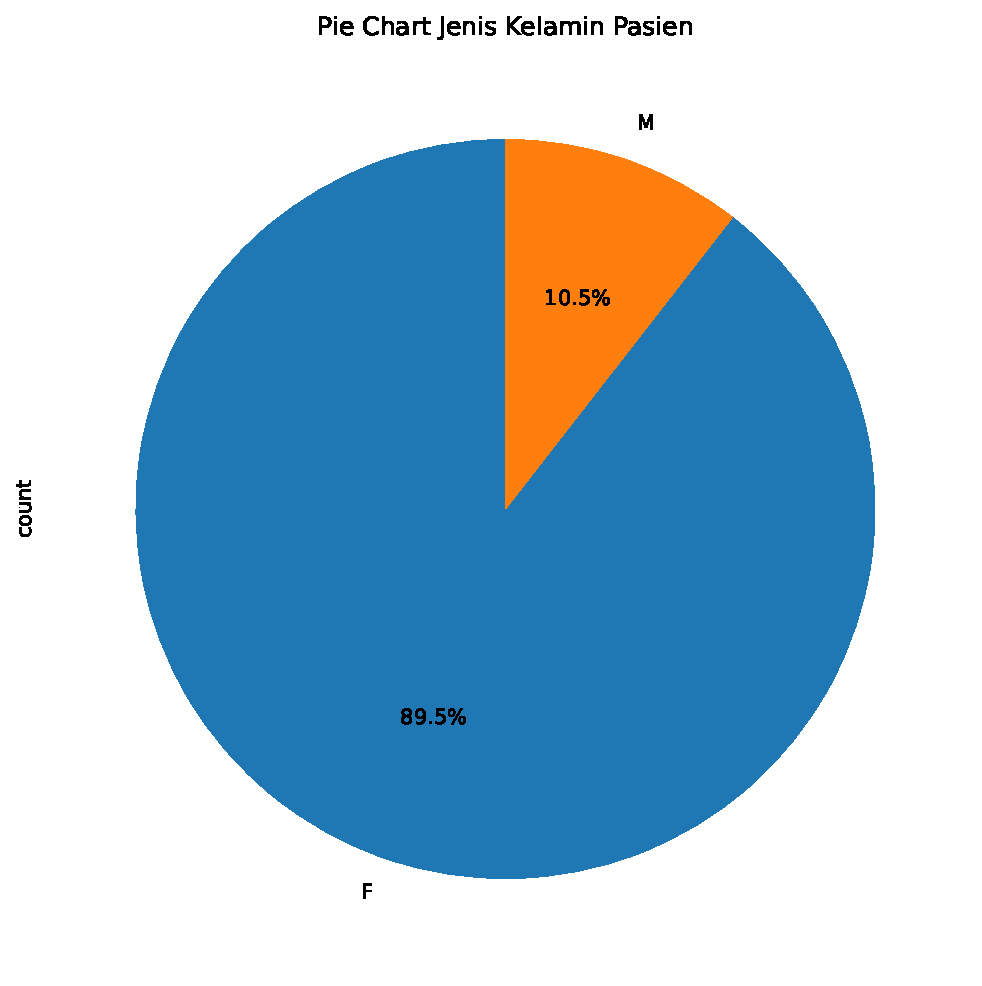
\includegraphics{index_files/figure-pdf/cell-7-output-1.pdf}

}

\end{figure}

Dari visualisasi Pie Chart Jenis Kelamin Pasien, terlihat bahwa proporsi
pasien perempuan (F) lebih dominan daripada pasien laki-laki (M).
Kesimpulan ini dapat diambil dari sebaran data yang menunjukkan bahwa
lebih banyak pasien yang dicatat dalam dataset memiliki jenis kelamin
perempuan daripada jenis kelamin laki-laki.

\hypertarget{visual-tentang-seberapa-pengaruh-cirrhosis-patient-pada-umur-tertent}{%
\subsection*{Visual tentang seberapa pengaruh Cirrhosis Patient pada
umur
tertent}\label{visual-tentang-seberapa-pengaruh-cirrhosis-patient-pada-umur-tertent}}
\addcontentsline{toc}{subsection}{Visual tentang seberapa pengaruh
Cirrhosis Patient pada umur tertent}

\begin{Shaded}
\begin{Highlighting}[]
\ImportTok{import}\NormalTok{ seaborn }\ImportTok{as}\NormalTok{ sns}
\NormalTok{plt.figure(figsize}\OperatorTok{=}\NormalTok{(}\DecValTok{10}\NormalTok{, }\DecValTok{6}\NormalTok{))}
\NormalTok{sns.histplot(df[}\StringTok{\textquotesingle{}Age\textquotesingle{}}\NormalTok{], bins}\OperatorTok{=}\DecValTok{30}\NormalTok{, kde}\OperatorTok{=}\VariableTok{True}\NormalTok{)}
\NormalTok{plt.title(}\StringTok{\textquotesingle{}Distribusi Umur Pasien\textquotesingle{}}\NormalTok{)}
\NormalTok{plt.xlabel(}\StringTok{\textquotesingle{}Umur\textquotesingle{}}\NormalTok{)}
\NormalTok{plt.ylabel(}\StringTok{\textquotesingle{}banyaknya pasien\textquotesingle{}}\NormalTok{)}
\NormalTok{plt.show()}

\NormalTok{plt.figure(figsize}\OperatorTok{=}\NormalTok{(}\DecValTok{10}\NormalTok{, }\DecValTok{6}\NormalTok{))}
\NormalTok{sns.boxplot(x}\OperatorTok{=}\StringTok{\textquotesingle{}Age\textquotesingle{}}\NormalTok{, y}\OperatorTok{=}\StringTok{\textquotesingle{}Status\textquotesingle{}}\NormalTok{, data}\OperatorTok{=}\NormalTok{df)}
\NormalTok{plt.title(}\StringTok{\textquotesingle{}Hubungan antara Umur dan Status Pasien\textquotesingle{}}\NormalTok{)}
\NormalTok{plt.xlabel(}\StringTok{\textquotesingle{}Status Pasien\textquotesingle{}}\NormalTok{)}
\NormalTok{plt.ylabel(}\StringTok{\textquotesingle{}Umur\textquotesingle{}}\NormalTok{)}
\NormalTok{plt.show()}
\end{Highlighting}
\end{Shaded}

\begin{figure}[H]

{\centering 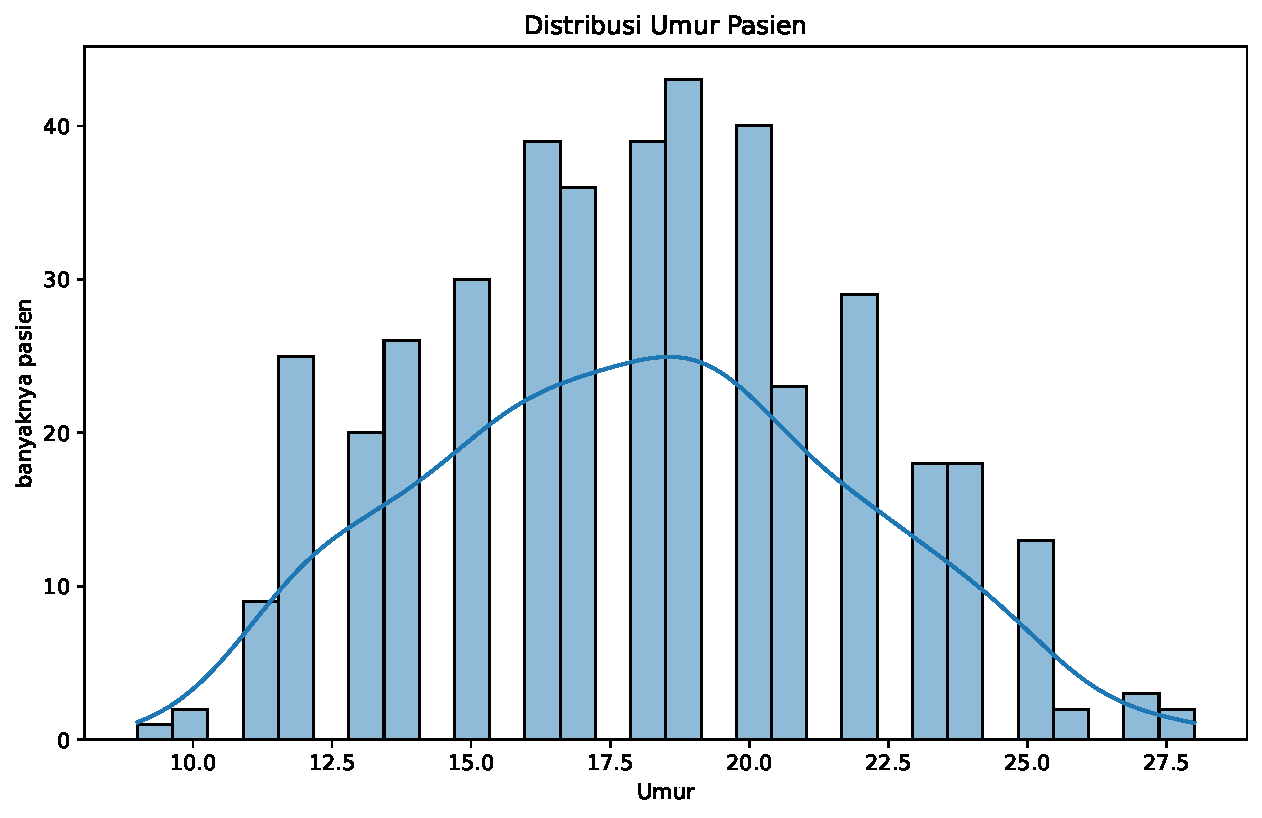
\includegraphics{index_files/figure-pdf/cell-8-output-1.pdf}

}

\end{figure}

\begin{figure}[H]

{\centering 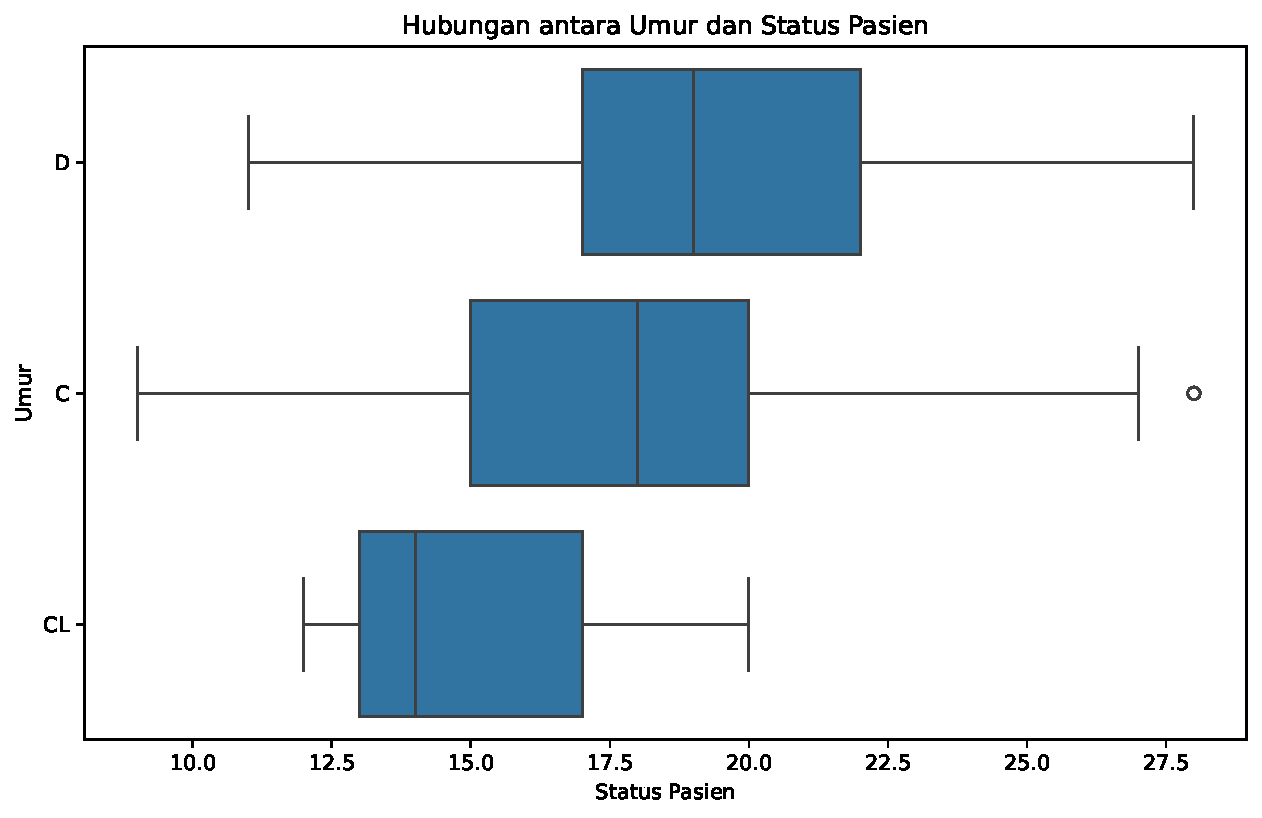
\includegraphics{index_files/figure-pdf/cell-8-output-2.pdf}

}

\end{figure}

\begin{enumerate}
\def\labelenumi{\arabic{enumi}.}
\item
  Rentang Usia Remaja (17-20 tahun): Pada rentang usia ini, terlihat
  adanya peningkatan signifikan dalam Cirrhosis Patient . Hal ini dapat
  menunjukkan bahwa remaja dalam kelompok usia ini mungkin memiliki
  faktor risiko tertentu yang berkontribusi pada prediksi penyakit hati.
  Status Pasien pada Usia 12-15 Tahun:
\item
  Prediksi status C (censored) yang lebih dominan pada kelompok usia
  12-15 tahun mungkin menunjukkan adanya kecenderungan untuk peristiwa
  yang tidak dapat diamati secara penuh. Ini bisa disebabkan oleh data
  yang tidak lengkap atau informasi yang tidak tersedia setelah periode
  pengamatan tertentu. Status Pasien pada Usia 14-20 Tahun:
\item
  Rentang usia 14-20 tahun menunjukkan kecenderungan prediksi status CL
  (censored karena transplantasi hati). Ini mungkin menandakan bahwa di
  dalam kelompok ini, pasien memiliki perawatan atau intervensi medis
  tertentu yang menyebabkan data pengamatan terhenti, seperti
  transplantasi hati. Status Pasien pada Usia 16-22 Tahun:
\item
  Pada usia ini, prediksi status D (kematian) mulai muncul lebih sering.
  Hal ini bisa menunjukkan tingkat keparahan penyakit atau faktor risiko
  tambahan yang dapat memengaruhi hasil pasien pada kelompok usia
  tersebut.
\end{enumerate}

\hypertarget{informasi-pada-label-dataset}{%
\section*{Informasi pada label
dataset}\label{informasi-pada-label-dataset}}
\addcontentsline{toc}{section}{Informasi pada label dataset}

\markright{Informasi pada label dataset}

\begin{Shaded}
\begin{Highlighting}[]
\NormalTok{target\_counts }\OperatorTok{=}\NormalTok{ df[}\StringTok{\textquotesingle{}Status\textquotesingle{}}\NormalTok{].value\_counts()}
\NormalTok{jumlah\_kategori }\OperatorTok{=}\NormalTok{ df[}\StringTok{\textquotesingle{}Status\textquotesingle{}}\NormalTok{].nunique()}

\BuiltInTok{print}\NormalTok{(}\StringTok{"Jumlah kategori pada target:"}\NormalTok{, jumlah\_kategori)}
\BuiltInTok{print}\NormalTok{(target\_counts)}
\end{Highlighting}
\end{Shaded}

\begin{verbatim}
Jumlah kategori pada target: 3
Status
C     232
D     161
CL     25
Name: count, dtype: int64
\end{verbatim}

Disini pada label mempunya 3 kelas yaitu: - C (Censored): Artinya pasien
tidak mengalami peristiwa akhir atau mati selama periode pengamatan.
Data pasien tersebut ``censored'' karena tidak ada informasi akhir yang
tersedia. - CL (Censored due to liver tx) Artinya pasien tidak mengalami
peristiwa akhir karena censored dan peristiwa censored tersebut terjadi
karena pasien menjalani transplantasi hati. - D (Death): Artinya pasien
mengalami kematian sebagai peristiwa akhir selama periode pengamatan

diatas bahwa data terbanyak yaitu categori C

Perbedaan C dan CL yaitu \textbf{C keterangannya tidak peristiwa akhir
atau mati tapi tidak melakukan transplantasi hati sedangkan CL juga
tidak ada tanda tanda peristiwa akhir tetapi harus menjalankan
transplantasi hati untuk menggantikan hati yang rusak}

\begin{Shaded}
\begin{Highlighting}[]
\NormalTok{X }\OperatorTok{=}\NormalTok{ df.drop([}\StringTok{\textquotesingle{}Status\textquotesingle{}}\NormalTok{,}\StringTok{\textquotesingle{}ID\textquotesingle{}}\NormalTok{], axis}\OperatorTok{=}\DecValTok{1}\NormalTok{)}
\NormalTok{y }\OperatorTok{=}\NormalTok{ df[}\StringTok{"Status"}\NormalTok{]}
\end{Highlighting}
\end{Shaded}

Memisahkan antara fitur dengan label

\hypertarget{seleksi-fitur}{%
\section*{Seleksi fitur}\label{seleksi-fitur}}
\addcontentsline{toc}{section}{Seleksi fitur}

\markright{Seleksi fitur}

sebelum melakukan preprocessing data alangkah baiknya untuk
menyeleksikan fitur fitur yang menurut kita adalah fitur yang tidak
berpengaruh terhadap dataset dan mengurangi beban dataset agar tidak
menyebabkan overfitting

\begin{Shaded}
\begin{Highlighting}[]
\NormalTok{X[}\StringTok{\textquotesingle{}Drug\textquotesingle{}}\NormalTok{] }\OperatorTok{=}\NormalTok{ X[}\StringTok{\textquotesingle{}Drug\textquotesingle{}}\NormalTok{].astype(}\StringTok{\textquotesingle{}category\textquotesingle{}}\NormalTok{).cat.codes}
\NormalTok{X[}\StringTok{\textquotesingle{}Ascites\textquotesingle{}}\NormalTok{] }\OperatorTok{=}\NormalTok{ X[}\StringTok{\textquotesingle{}Ascites\textquotesingle{}}\NormalTok{].astype(}\StringTok{\textquotesingle{}category\textquotesingle{}}\NormalTok{).cat.codes}
\NormalTok{X[}\StringTok{\textquotesingle{}Hepatomegaly\textquotesingle{}}\NormalTok{] }\OperatorTok{=}\NormalTok{ X[}\StringTok{\textquotesingle{}Hepatomegaly\textquotesingle{}}\NormalTok{].astype(}\StringTok{\textquotesingle{}category\textquotesingle{}}\NormalTok{).cat.codes}
\NormalTok{X[}\StringTok{\textquotesingle{}Spiders\textquotesingle{}}\NormalTok{] }\OperatorTok{=}\NormalTok{ X[}\StringTok{\textquotesingle{}Spiders\textquotesingle{}}\NormalTok{].astype(}\StringTok{\textquotesingle{}category\textquotesingle{}}\NormalTok{).cat.codes}
\NormalTok{X[}\StringTok{\textquotesingle{}Stage\textquotesingle{}}\NormalTok{] }\OperatorTok{=}\NormalTok{ X[}\StringTok{\textquotesingle{}Stage\textquotesingle{}}\NormalTok{].astype(}\StringTok{\textquotesingle{}category\textquotesingle{}}\NormalTok{).cat.codes}
\NormalTok{X[}\StringTok{\textquotesingle{}Sex\textquotesingle{}}\NormalTok{] }\OperatorTok{=}\NormalTok{ X[}\StringTok{\textquotesingle{}Sex\textquotesingle{}}\NormalTok{].astype(}\StringTok{\textquotesingle{}category\textquotesingle{}}\NormalTok{).cat.codes}
\NormalTok{X[}\StringTok{\textquotesingle{}Edema\textquotesingle{}}\NormalTok{] }\OperatorTok{=}\NormalTok{ X[}\StringTok{\textquotesingle{}Edema\textquotesingle{}}\NormalTok{].astype(}\StringTok{\textquotesingle{}category\textquotesingle{}}\NormalTok{).cat.codes}
\ImportTok{from}\NormalTok{ sklearn.feature\_selection }\ImportTok{import}\NormalTok{ SelectKBest, f\_classif}


\NormalTok{selector }\OperatorTok{=}\NormalTok{ SelectKBest(score\_func}\OperatorTok{=}\NormalTok{f\_classif, k}\OperatorTok{=}\DecValTok{18}\NormalTok{)  }
\NormalTok{selector.fit(X, y)}

\NormalTok{selected\_features }\OperatorTok{=}\NormalTok{ selector.get\_support(indices}\OperatorTok{=}\VariableTok{True}\NormalTok{)}

\NormalTok{feature\_names }\OperatorTok{=}\NormalTok{ X.columns}


\NormalTok{selected\_feature\_names }\OperatorTok{=}\NormalTok{ [feature\_names[i] }\ControlFlowTok{for}\NormalTok{ i }\KeywordTok{in}\NormalTok{ selected\_features]}

\NormalTok{scores }\OperatorTok{=}\NormalTok{ selector.scores\_[selected\_features]}


\NormalTok{plt.figure(figsize}\OperatorTok{=}\NormalTok{(}\DecValTok{10}\NormalTok{, }\DecValTok{6}\NormalTok{))}
\NormalTok{plt.bar(selected\_feature\_names, scores, color}\OperatorTok{=}\StringTok{\textquotesingle{}skyblue\textquotesingle{}}\NormalTok{)}
\NormalTok{plt.xlabel(}\StringTok{\textquotesingle{}Fitur\textquotesingle{}}\NormalTok{)}
\NormalTok{plt.ylabel(}\StringTok{\textquotesingle{}Skor Statistik\textquotesingle{}}\NormalTok{)}
\NormalTok{plt.title(}\StringTok{\textquotesingle{}Skor Statistik untuk Fitur{-}Fitur Terpilih\textquotesingle{}}\NormalTok{)}
\NormalTok{plt.xticks(rotation}\OperatorTok{=}\DecValTok{45}\NormalTok{)}
\NormalTok{plt.tight\_layout()}

\CommentTok{\# Menampilkan grafik}
\NormalTok{plt.show()}
\end{Highlighting}
\end{Shaded}

\begin{figure}[H]

{\centering 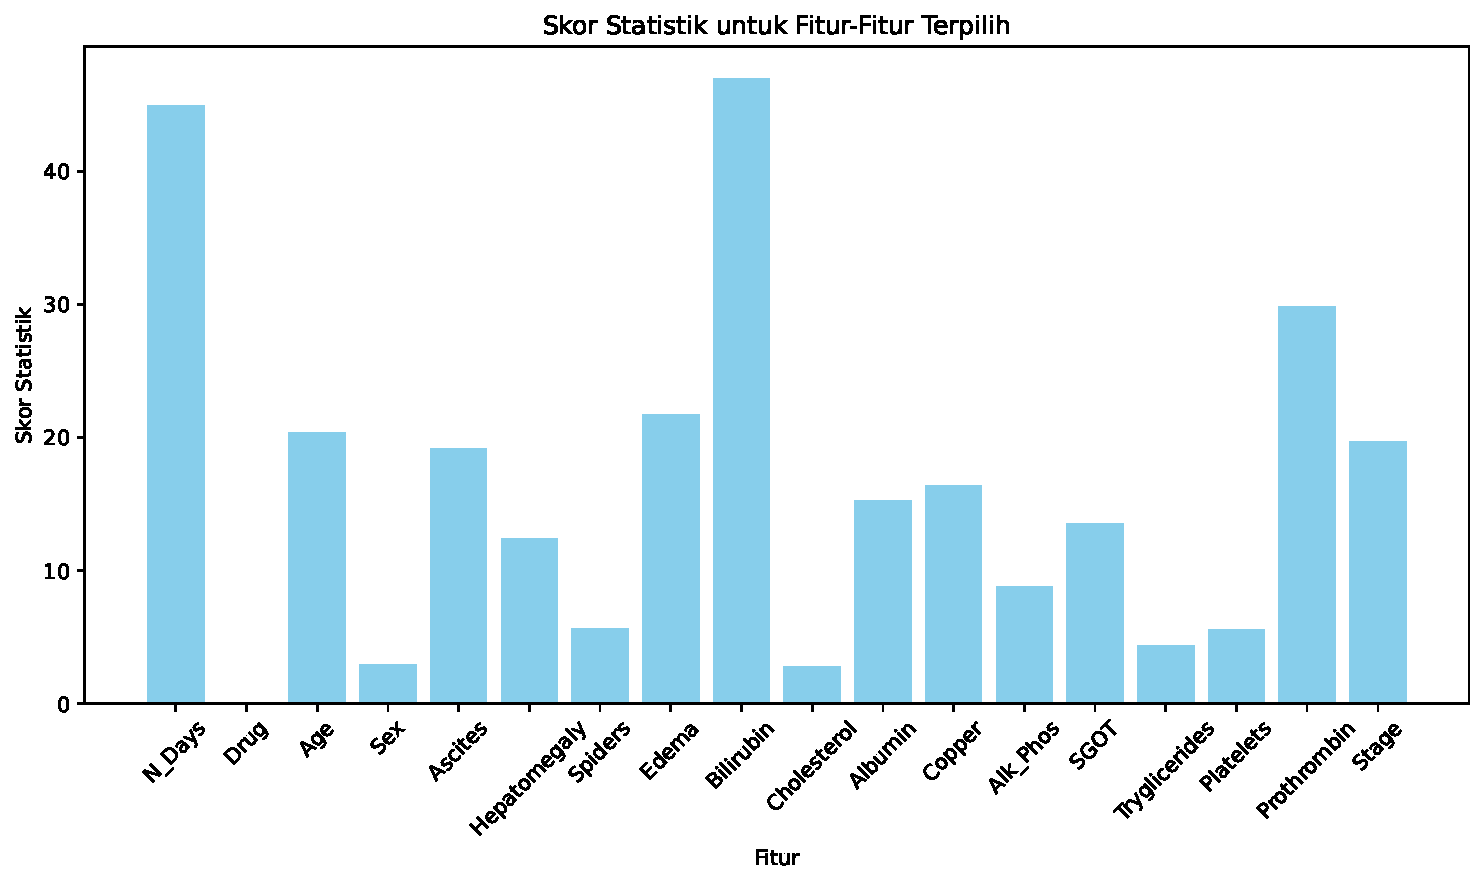
\includegraphics{index_files/figure-pdf/cell-11-output-1.pdf}

}

\end{figure}

Disini saya menggunakan sckit learn untuk melakukan selection pada fitur
- yang pertama saya menentukan banyaknya fitur terdapat N = banyak
fitur, fitur yang ada didataset adalah 19 fitur - Jumlah fitur terbaik
yang terpilih disesuaikan dengan nilai K di atas - ambil data data pada
setiap fitur menggunakan funtion colomns dan nama pada fitur akan
dimasukan kedalam selected\_feature\_names - lalu proses melakukan
perhitungan statistik ANOVA dengan rumus

\[
F = \frac{MSB}{MSW}
\] MSB atau mean square antar kelompok (mean square between groups).
dapat dari rumus ini :

\[
MSB = \frac{\sum_{i=1}^{k} n_i (\bar{X}_i - \bar{X}_{\text{total}})^2}{k - 1}
\] dan MSW atau mean square dalam kelompok (mean square within groups)

\[
MSW = \frac{\sum_{i=1}^{k} \sum_{j=1}^{n_i} (X_{ij} - \bar{X}_i)^2}{N - k}
\] Untuk hasil akhirnya saya menghapus 8 fitur yang menurut saya tidak
akan berpengaruh terhadap dataset saya

\begin{Shaded}
\begin{Highlighting}[]
\NormalTok{X }\OperatorTok{=}\NormalTok{ df.drop([}\StringTok{\textquotesingle{}N\_Days\textquotesingle{}}\NormalTok{,}\StringTok{\textquotesingle{}ID\textquotesingle{}}\NormalTok{,}\StringTok{\textquotesingle{}Status\textquotesingle{}}\NormalTok{,}\StringTok{\textquotesingle{}Drug\textquotesingle{}}\NormalTok{,}\StringTok{\textquotesingle{}Sex\textquotesingle{}}\NormalTok{,}\StringTok{\textquotesingle{}Spiders\textquotesingle{}}\NormalTok{,}\StringTok{\textquotesingle{}Cholesterol\textquotesingle{}}\NormalTok{,}\StringTok{\textquotesingle{}Tryglicerides\textquotesingle{}}\NormalTok{,}\StringTok{\textquotesingle{}Platelets\textquotesingle{}}\NormalTok{], axis}\OperatorTok{=}\DecValTok{1}\NormalTok{)}
\NormalTok{X}
\end{Highlighting}
\end{Shaded}

\begin{longtable}[]{@{}llllllllllll@{}}
\toprule\noalign{}
& Age & Ascites & Hepatomegaly & Edema & Bilirubin & Albumin & Copper &
Alk\_Phos & SGOT & Prothrombin & Stage \\
\midrule\noalign{}
\endhead
\bottomrule\noalign{}
\endlastfoot
0 & 21 & Y & Y & Y & 14.5 & 2.60 & 156.0 & 1718.0 & 137.95 & 12.2 &
4.0 \\
1 & 20 & N & Y & N & 1.1 & 4.14 & 54.0 & 7394.8 & 113.52 & 10.6 & 3.0 \\
2 & 25 & N & N & S & 1.4 & 3.48 & 210.0 & 516.0 & 96.10 & 12.0 & 4.0 \\
3 & 19 & N & Y & S & 1.8 & 2.54 & 64.0 & 6121.8 & 60.63 & 10.3 & 4.0 \\
4 & 13 & N & Y & N & 3.4 & 3.53 & 143.0 & 671.0 & 113.15 & 10.9 & 3.0 \\
... & ... & ... & ... & ... & ... & ... & ... & ... & ... & ... & ... \\
413 & 24 & N & Y & N & 1.2 & 2.96 & 186.0 & 2115.0 & 136.00 & 10.9 &
3.0 \\
414 & 14 & N & Y & N & 0.9 & 3.83 & 186.0 & 2115.0 & 136.00 & 11.2 &
4.0 \\
415 & 20 & N & Y & N & 1.6 & 3.42 & 186.0 & 2115.0 & 136.00 & 9.9 &
3.0 \\
416 & 21 & N & Y & N & 0.8 & 3.75 & 186.0 & 2115.0 & 136.00 & 10.4 &
3.0 \\
417 & 19 & N & Y & N & 0.7 & 3.29 & 186.0 & 2115.0 & 136.00 & 10.6 &
4.0 \\
\end{longtable}

\hypertarget{mengganti-categori-menjadi-numerik}{%
\section*{Mengganti categori menjadi
numerik}\label{mengganti-categori-menjadi-numerik}}
\addcontentsline{toc}{section}{Mengganti categori menjadi numerik}

\markright{Mengganti categori menjadi numerik}

Sebelum melakukan preprosessing pada dataset saya diketahui memiliki
categori yang harus diganti menjadi numerik, maka saya gunakan code
seperti dibawah :

\begin{Shaded}
\begin{Highlighting}[]
\NormalTok{X[}\StringTok{\textquotesingle{}Ascites\textquotesingle{}}\NormalTok{] }\OperatorTok{=}\NormalTok{ X[}\StringTok{\textquotesingle{}Ascites\textquotesingle{}}\NormalTok{].astype(}\StringTok{\textquotesingle{}category\textquotesingle{}}\NormalTok{).cat.codes}
\NormalTok{X[}\StringTok{\textquotesingle{}Hepatomegaly\textquotesingle{}}\NormalTok{] }\OperatorTok{=}\NormalTok{ X[}\StringTok{\textquotesingle{}Hepatomegaly\textquotesingle{}}\NormalTok{].astype(}\StringTok{\textquotesingle{}category\textquotesingle{}}\NormalTok{).cat.codes}
\NormalTok{X[}\StringTok{\textquotesingle{}Edema\textquotesingle{}}\NormalTok{] }\OperatorTok{=}\NormalTok{ X[}\StringTok{\textquotesingle{}Edema\textquotesingle{}}\NormalTok{].astype(}\StringTok{\textquotesingle{}category\textquotesingle{}}\NormalTok{).cat.codes}
\NormalTok{X}
\end{Highlighting}
\end{Shaded}

\begin{longtable}[]{@{}llllllllllll@{}}
\toprule\noalign{}
& Age & Ascites & Hepatomegaly & Edema & Bilirubin & Albumin & Copper &
Alk\_Phos & SGOT & Prothrombin & Stage \\
\midrule\noalign{}
\endhead
\bottomrule\noalign{}
\endlastfoot
0 & 21 & 1 & 1 & 2 & 14.5 & 2.60 & 156.0 & 1718.0 & 137.95 & 12.2 &
4.0 \\
1 & 20 & 0 & 1 & 0 & 1.1 & 4.14 & 54.0 & 7394.8 & 113.52 & 10.6 & 3.0 \\
2 & 25 & 0 & 0 & 1 & 1.4 & 3.48 & 210.0 & 516.0 & 96.10 & 12.0 & 4.0 \\
3 & 19 & 0 & 1 & 1 & 1.8 & 2.54 & 64.0 & 6121.8 & 60.63 & 10.3 & 4.0 \\
4 & 13 & 0 & 1 & 0 & 3.4 & 3.53 & 143.0 & 671.0 & 113.15 & 10.9 & 3.0 \\
... & ... & ... & ... & ... & ... & ... & ... & ... & ... & ... & ... \\
413 & 24 & 0 & 1 & 0 & 1.2 & 2.96 & 186.0 & 2115.0 & 136.00 & 10.9 &
3.0 \\
414 & 14 & 0 & 1 & 0 & 0.9 & 3.83 & 186.0 & 2115.0 & 136.00 & 11.2 &
4.0 \\
415 & 20 & 0 & 1 & 0 & 1.6 & 3.42 & 186.0 & 2115.0 & 136.00 & 9.9 &
3.0 \\
416 & 21 & 0 & 1 & 0 & 0.8 & 3.75 & 186.0 & 2115.0 & 136.00 & 10.4 &
3.0 \\
417 & 19 & 0 & 1 & 0 & 0.7 & 3.29 & 186.0 & 2115.0 & 136.00 & 10.6 &
4.0 \\
\end{longtable}

diatas terdapat cara untuk menggantikan sebuah type kategori menjadi
numerik, terdapat fungsi yang saya pakai :

\begin{itemize}
\item
  astype(`category') , funtion tersebut untuk memberi tahu bahwa pada
  fitur tersebut adalah type category
\item
  cat.codes untuk mengubah category menjadi numerik, Bilangan bulat yang
  diberikan dimulai dari 0 dan terus bertambah seiring dengan munculnya
  nilai kategori yang baru. contohnya pada fitur Sex mempunyai 2
  category yaitu wanita dan lelaki, maka wanita akan diganti menjadi 0
  dan lelaki akan menjadi 1
\end{itemize}

\bookmarksetup{startatroot}

\hypertarget{preprocessing-data}{%
\chapter*{Preprocessing data}\label{preprocessing-data}}
\addcontentsline{toc}{chapter}{Preprocessing data}

\markboth{Preprocessing data}{Preprocessing data}

\hypertarget{split-data-menjadi-train-data-dan-test-data}{%
\section*{Split data menjadi train data dan test
data}\label{split-data-menjadi-train-data-dan-test-data}}
\addcontentsline{toc}{section}{Split data menjadi train data dan test
data}

\markright{Split data menjadi train data dan test data}

train\_test\_split adalah suatu fungsi dalam library scikit-learn yang
digunakan untuk membagi dataset menjadi dua set, yaitu set pelatihan
(training set) dan set pengujian (testing set). Pemisahan ini bertujuan
untuk melakukan pelatihan model pada set pelatihan dan menguji kinerja
model pada set pengujian. Fungsi ini sangat umum digunakan dalam proses
machine learning untuk menghindari overfitting dan mengevaluasi
kemampuan generalisasi dari model yang telah dilatih

\begin{enumerate}
\def\labelenumi{\arabic{enumi}.}
\item
  test\_size (opsional): Menentukan ukuran set pengujian sebagai
  proporsi dari seluruh dataset. Nilai ini bisa berupa pecahan
  (misalnya, 0.2 untuk 20\%) atau bilangan bulat yang menyatakan jumlah
  sampel yang akan ditempatkan di set pengujian.
\item
  random\_state (opsional): Digunakan untuk mengontrol randomization
  selama pembagian dataset. Jika nilai ini diberikan, pemisahan dataset
  akan tetap konsisten setiap kali fungsi ini dijalankan
\end{enumerate}

\hypertarget{normalisasi-data}{%
\section*{Normalisasi data}\label{normalisasi-data}}
\addcontentsline{toc}{section}{Normalisasi data}

\markright{Normalisasi data}

Setelah melakukan understanding data maka melakukan preprocessing yang
dimana data akan di jadikan antara 0 sampai 1

\begin{Shaded}
\begin{Highlighting}[]
\ImportTok{from}\NormalTok{ sklearn.model\_selection }\ImportTok{import}\NormalTok{ train\_test\_split, cross\_val\_score}
\ImportTok{from}\NormalTok{ sklearn.preprocessing }\ImportTok{import}\NormalTok{ MinMaxScaler}
\NormalTok{X\_train, X\_test, y\_train, y\_test }\OperatorTok{=}\NormalTok{ train\_test\_split(X, y, test\_size}\OperatorTok{=}\FloatTok{0.2}\NormalTok{, random\_state}\OperatorTok{=}\DecValTok{42}\NormalTok{)}

\NormalTok{scaler }\OperatorTok{=}\NormalTok{ MinMaxScaler()}
\NormalTok{X\_train\_scaler }\OperatorTok{=}\NormalTok{ scaler.fit\_transform(X\_train)}
\NormalTok{X\_test\_scaler }\OperatorTok{=}\NormalTok{ scaler.transform(X\_test)}
\NormalTok{x }\OperatorTok{=}\NormalTok{ pd.DataFrame(X\_train,columns}\OperatorTok{=}\NormalTok{X.columns)}
\NormalTok{x}
\end{Highlighting}
\end{Shaded}

\begin{longtable}[]{@{}llllllllllll@{}}
\toprule\noalign{}
& Age & Ascites & Hepatomegaly & Edema & Bilirubin & Albumin & Copper &
Alk\_Phos & SGOT & Prothrombin & Stage \\
\midrule\noalign{}
\endhead
\bottomrule\noalign{}
\endlastfoot
336 & 20 & 0 & 1 & 0 & 1.8 & 3.64 & 186.0 & 2115.0 & 136.00 & 10.0 &
3.0 \\
31 & 19 & 0 & 1 & 0 & 1.8 & 3.34 & 101.0 & 7277.0 & 82.56 & 10.6 &
4.0 \\
84 & 17 & 0 & 1 & 0 & 2.1 & 3.48 & 58.0 & 2045.0 & 89.90 & 11.5 & 4.0 \\
287 & 17 & 0 & 1 & 1 & 8.7 & 3.89 & 107.0 & 637.0 & 117.00 & 9.6 &
2.0 \\
317 & 15 & 0 & 1 & 0 & 0.7 & 3.68 & 186.0 & 2115.0 & 136.00 & 9.5 &
2.0 \\
... & ... & ... & ... & ... & ... & ... & ... & ... & ... & ... & ... \\
71 & 11 & 0 & 0 & 0 & 0.5 & 3.54 & 51.0 & 1243.0 & 122.45 & 10.0 &
3.0 \\
106 & 22 & 0 & 0 & 0 & 0.6 & 4.03 & 10.0 & 648.0 & 71.30 & 17.1 & 1.0 \\
270 & 18 & 0 & 1 & 0 & 1.0 & 3.50 & 94.0 & 955.0 & 111.00 & 9.7 & 3.0 \\
348 & 19 & 0 & 1 & 0 & 1.4 & 3.82 & 186.0 & 2115.0 & 136.00 & 10.3 &
2.0 \\
102 & 17 & 1 & 1 & 2 & 2.5 & 3.67 & 57.0 & 1273.0 & 119.35 & 11.1 &
4.0 \\
\end{longtable}

dengan menggunakan minmaxScaller untuk menormalisasi data , dan
menggunakan train\_test\_split untuk mendapatkan data training dan data
testing

rumus MinmaxScaler:

\[
\text{Scaled Value} = \frac{\text{Original Value} - \text{Min}}{\text{Max} - \text{Min}}
\] - Original Value adalah nilai asli dari fitur.

\begin{itemize}
\item
  Min adalah nilai minimum dari fitur.
\item
  Max adalah nilai maksimum dari fitur.
\end{itemize}

\begin{enumerate}
\def\labelenumi{\arabic{enumi}.}
\item
  fit\_transform Fungsinya ini menghitung parameter normalisasi dari
  dataset (seperti nilai minimum dan maksimum) dan kemudian
  mengaplikasikan normalisasi pada dataset tersebut. Fungsi ini berguna
  untuk menghitung parameter normalisasi berdasarkan data pelatihan dan
  sekaligus menerapkan normalisasi tersebut.
\item
  Setelah kita telah menggunakan fit\_transform pada data pelatihan,
  kita dapat menggunakan metode transform pada data pengujian (dan data
  lainnya yang ingin dinormalisasi) menggunakan parameter normalisasi
  yang telah dihitung sebelumnya. Metode ini hanya melakukan normalisasi
  tanpa perlu menghitung parameter normalisasi lagi.
\end{enumerate}

\bookmarksetup{startatroot}

\hypertarget{modeling-data}{%
\chapter*{Modeling data}\label{modeling-data}}
\addcontentsline{toc}{chapter}{Modeling data}

\markboth{Modeling data}{Modeling data}

\hypertarget{melatih-model-menggunakan-random-forest}{%
\section*{Melatih Model menggunakan Random
Forest}\label{melatih-model-menggunakan-random-forest}}
\addcontentsline{toc}{section}{Melatih Model menggunakan Random Forest}

\markright{Melatih Model menggunakan Random Forest}

Random Forest adalah sebuah algoritma machine learning yang digunakan
untuk tugas klasifikasi, regresi, dan pengurangan dimensi. Ini merupakan
jenis algoritma ensemble, yang menggabungkan beberapa model untuk
meningkatkan kinerja dan kestabilan prediksi. Algoritma Random Forest
membangun beberapa pohon keputusan selama pelatihan dan menggabungkan
hasil prediksi dari pohon-pohon tersebut untuk membuat prediksi yang
lebih akurat dan stabil

\begin{Shaded}
\begin{Highlighting}[]
\ImportTok{from}\NormalTok{ sklearn.ensemble }\ImportTok{import}\NormalTok{ RandomForestClassifier}
\ImportTok{from}\NormalTok{ sklearn.metrics }\ImportTok{import}\NormalTok{ accuracy\_score}
\CommentTok{\# Buat model Random Forest}
\NormalTok{random\_forest\_model }\OperatorTok{=}\NormalTok{ RandomForestClassifier(n\_estimators}\OperatorTok{=}\DecValTok{100}\NormalTok{)}
\CommentTok{\# Latih model}
\NormalTok{random\_forest\_model.fit(X\_train, y\_train)}
\CommentTok{\# Prediksi dengan model}
\NormalTok{random\_forest\_predictions }\OperatorTok{=}\NormalTok{ random\_forest\_model.predict(X\_test)}
\CommentTok{\# Evaluasi kinerja model}
\NormalTok{random\_forest\_accuracy }\OperatorTok{=}\NormalTok{ accuracy\_score(y\_test, random\_forest\_predictions)}
\end{Highlighting}
\end{Shaded}

alasan mengapa menggunakan Random Forest Dengan mempertimbangkan acak
dan menggunakan banyak pohon, Random Forest dapat mengurangi risiko
overfitting pada data pelatihan.

rumus Random forest

\begin{enumerate}
\def\labelenumi{\arabic{enumi}.}
\item
  Prediksi pada Pohon Keputusan \[
  \text{Prediction}_{\text{tree}} = \text{MajorityClass}(\text{Samples in Leaf})
  \]
\item
  Aggregasi Prediksi dari Semua Pohon (Klasifikasi) \[
  \text{Final Prediction}_{\text{RF}} = \text{MajorityClass}(\text{Predictions from all Trees})
  \]
\item
  Aggregasi Prediksi dari Semua Pohon (Regresi) \[
  \text{Final Prediction}_{\text{RF}} = \text{Average}(\text{Predictions from all Trees})
  \]
\end{enumerate}

\hypertarget{melatih-data-menggunakan-logistic-regression}{%
\section*{Melatih data menggunakan Logistic
Regression}\label{melatih-data-menggunakan-logistic-regression}}
\addcontentsline{toc}{section}{Melatih data menggunakan Logistic
Regression}

\markright{Melatih data menggunakan Logistic Regression}

Logistic Regression (Regresi Logistik) adalah algoritma machine learning
yang digunakan untuk tugas klasifikasi. Meskipun memiliki kata
``regresi'' dalam namanya, logistic regression sebenarnya digunakan
untuk masalah klasifikasi biner, di mana tujuannya adalah memprediksi
kelas target yang memiliki dua kemungkinan nilai (biasanya 0 atau 1).

\[
P(Y=1) = \frac{1}{1 + e^{-(\beta_0 + \beta_1 X_1 + \beta_2 X_2 + \ldots + \beta_n X_n)}}
\]

\begin{itemize}
\tightlist
\item
  P(Y=1) adalah probabilitas kejadian
\item
  Y sama dengan 1.
\item
  e adalah basis logaritma natural.
\item
  b adalah bobot .
\item
  X adalah data .
\end{itemize}

\begin{Shaded}
\begin{Highlighting}[]
\ImportTok{from}\NormalTok{ sklearn.linear\_model }\ImportTok{import}\NormalTok{ LogisticRegression}
\NormalTok{model }\OperatorTok{=}\NormalTok{ LogisticRegression()}

\CommentTok{\# Latih model}
\NormalTok{model.fit(X\_train\_scaler, y\_train)}

\CommentTok{\# Prediksi dengan model}
\NormalTok{logistic\_regression\_predictions }\OperatorTok{=}\NormalTok{ model.predict(X\_test)}

\CommentTok{\# Evaluasi kinerja model}
\NormalTok{logistic\_regression\_accuracy }\OperatorTok{=}\NormalTok{ accuracy\_score(y\_test, logistic\_regression\_predictions)}
\end{Highlighting}
\end{Shaded}

\begin{verbatim}
/cloud/python/lib/python3.8/site-packages/sklearn/base.py:458: UserWarning: X has feature names, but LogisticRegression was fitted without feature names
  warnings.warn(
\end{verbatim}

\hypertarget{melatih-data-menggunakan-percepton}{%
\section*{Melatih data menggunakan
Percepton}\label{melatih-data-menggunakan-percepton}}
\addcontentsline{toc}{section}{Melatih data menggunakan Percepton}

\markright{Melatih data menggunakan Percepton}

Perceptron adalah model dasar dalam machine learning yang digunakan
untuk tugas klasifikasi biner. Perceptron dirancang untuk memodelkan
neuron dalam otak manusia dan dapat digunakan untuk memisahkan dua kelas
dengan menarik garis pemisah linier. Namun, perceptron memiliki
keterbatasan dan biasanya digunakan sebagai dasar untuk model neural
network yang lebih kompleks.

\[
\text{Output} = \begin{cases} 
1 & \text{jika } \sum_{i=1}^{n} w_i x_i + b > 0 \\
0 & \text{lainnya}
\end{cases}
\]

\begin{Shaded}
\begin{Highlighting}[]
\ImportTok{from}\NormalTok{ sklearn.linear\_model }\ImportTok{import}\NormalTok{ Perceptron, SGDClassifier}
\CommentTok{\# Buat model Perceptron}
\NormalTok{perceptron\_model }\OperatorTok{=}\NormalTok{ Perceptron(max\_iter}\OperatorTok{=}\DecValTok{1000}\NormalTok{, random\_state}\OperatorTok{=}\DecValTok{42}\NormalTok{)}

\CommentTok{\# Latih model Perceptron}
\NormalTok{perceptron\_model.fit(X\_train\_scaler, y\_train)}

\CommentTok{\# Prediksi dengan model Perceptron}
\NormalTok{perceptron\_predictions }\OperatorTok{=}\NormalTok{ perceptron\_model.predict(X\_test)}

\CommentTok{\# Evaluasi kinerja model Perceptron}
\NormalTok{perceptron\_accuracy }\OperatorTok{=}\NormalTok{ accuracy\_score(y\_test, perceptron\_predictions)}
\end{Highlighting}
\end{Shaded}

\begin{verbatim}
/cloud/python/lib/python3.8/site-packages/sklearn/base.py:458: UserWarning: X has feature names, but Perceptron was fitted without feature names
  warnings.warn(
\end{verbatim}

\hypertarget{melatih-data-menggunakan-jaringan-saraf-tiruan}{%
\section*{Melatih data menggunakan Jaringan Saraf
Tiruan}\label{melatih-data-menggunakan-jaringan-saraf-tiruan}}
\addcontentsline{toc}{section}{Melatih data menggunakan Jaringan Saraf
Tiruan}

\markright{Melatih data menggunakan Jaringan Saraf Tiruan}

Jaringan Saraf Tiruan (JST) atau Neural Networks adalah bagian integral
dari machine learning. Neural networks terinspirasi oleh struktur dan
fungsi otak manusia dan dapat digunakan untuk menangani tugas-tugas
kompleks seperti klasifikasi, regresi, pengenalan pola, dan bahkan
pembelajaran tugas-tugas yang lebih kompleks

\begin{Shaded}
\begin{Highlighting}[]
\ImportTok{from}\NormalTok{ sklearn.neural\_network }\ImportTok{import}\NormalTok{ MLPClassifier}
\NormalTok{neural\_network\_model }\OperatorTok{=}\NormalTok{ MLPClassifier(hidden\_layer\_sizes}\OperatorTok{=}\NormalTok{(}\DecValTok{64}\NormalTok{, }\DecValTok{32}\NormalTok{), max\_iter}\OperatorTok{=}\DecValTok{1000}\NormalTok{, random\_state}\OperatorTok{=}\DecValTok{42}\NormalTok{)}

\CommentTok{\# Latih model}
\NormalTok{neural\_network\_model.fit(X\_train\_scaler, y\_train)}

\CommentTok{\# Prediksi dengan model}
\NormalTok{neural\_network\_predictions }\OperatorTok{=}\NormalTok{ neural\_network\_model.predict(X\_test)}

\CommentTok{\# Evaluasi kinerja model}
\NormalTok{neural\_network\_accuracy }\OperatorTok{=}\NormalTok{ accuracy\_score(y\_test, neural\_network\_predictions)}
\end{Highlighting}
\end{Shaded}

\begin{verbatim}
/cloud/python/lib/python3.8/site-packages/sklearn/neural_network/_multilayer_perceptron.py:691: ConvergenceWarning: Stochastic Optimizer: Maximum iterations (1000) reached and the optimization hasn't converged yet.
  warnings.warn(
/cloud/python/lib/python3.8/site-packages/sklearn/base.py:458: UserWarning: X has feature names, but MLPClassifier was fitted without feature names
  warnings.warn(
\end{verbatim}

\hypertarget{melatih-model-menggunakan-decision-tree}{%
\section*{Melatih Model menggunakan decision
tree}\label{melatih-model-menggunakan-decision-tree}}
\addcontentsline{toc}{section}{Melatih Model menggunakan decision tree}

\markright{Melatih Model menggunakan decision tree}

Decision tree (pohon keputusan) adalah model prediktif yang digunakan
dalam machine learning dan data mining. Model ini mengambil bentuk pohon
dengan setiap simpul (node) yang mewakili keputusan atau pengujian
terhadap suatu fitur, cabang (branch) yang mengarah ke simpul lainnya,
dan daun (leaf) yang memberikan hasil atau prediksi. Decision tree
digunakan untuk tugas klasifikasi dan regresi.

\[
\begin{equation}
\text{Jika } X_i \leq T \text{ maka cabang kiri, else cabang kanan}
\end{equation}
\]

\begin{Shaded}
\begin{Highlighting}[]
\ImportTok{from}\NormalTok{ sklearn.tree }\ImportTok{import}\NormalTok{ DecisionTreeClassifier}
\NormalTok{decision\_tree\_model }\OperatorTok{=}\NormalTok{ DecisionTreeClassifier()}
\CommentTok{\# Latih model}
\NormalTok{decision\_tree\_model.fit(X\_train, y\_train)}
\CommentTok{\# Prediksi dengan model}
\NormalTok{decision\_tree\_predictions }\OperatorTok{=}\NormalTok{ decision\_tree\_model.predict(X\_test)}
\CommentTok{\# Evaluasi kinerja model}
\NormalTok{decision\_tree\_accuracy }\OperatorTok{=}\NormalTok{ accuracy\_score(y\_test, decision\_tree\_predictions)}
\end{Highlighting}
\end{Shaded}

\bookmarksetup{startatroot}

\hypertarget{evaluasi}{%
\chapter*{Evaluasi}\label{evaluasi}}
\addcontentsline{toc}{chapter}{Evaluasi}

\markboth{Evaluasi}{Evaluasi}

\begin{Shaded}
\begin{Highlighting}[]
\BuiltInTok{print}\NormalTok{(}\StringTok{"Akurasi Random Forest:"}\NormalTok{, decision\_tree\_accuracy)}
\BuiltInTok{print}\NormalTok{(}\StringTok{"Akurasi Random Forest:"}\NormalTok{, random\_forest\_accuracy)}
\BuiltInTok{print}\NormalTok{(}\StringTok{"Akurasi Regresi Logistik:"}\NormalTok{, logistic\_regression\_accuracy)}
\BuiltInTok{print}\NormalTok{(}\StringTok{"Akurasi Perceptron:"}\NormalTok{, perceptron\_accuracy)}
\BuiltInTok{print}\NormalTok{(}\StringTok{"Akurasi neural\_network:"}\NormalTok{, neural\_network\_accuracy)}
\end{Highlighting}
\end{Shaded}

\begin{verbatim}
Akurasi Random Forest: 0.6785714285714286
Akurasi Random Forest: 0.75
Akurasi Regresi Logistik: 0.42857142857142855
Akurasi Perceptron: 0.42857142857142855
Akurasi neural_network: 0.42857142857142855
\end{verbatim}

Pada akurasi ini adalah paling tinggi di model yang lain, maka saya
memilih metode random forest, alasan lainnya mengapa menggunakan Random
Forest Dengan mempertimbangkan acak dan menggunakan banyak pohon, Random
Forest dapat mengurangi risiko overfitting pada data pelatihan

\begin{Shaded}
\begin{Highlighting}[]
\ImportTok{import}\NormalTok{ joblib}
\CommentTok{\# from sklearn.externals import joblib}
\NormalTok{joblib.dump(random\_forest\_model, }\StringTok{\textquotesingle{}model\_rf.joblib\textquotesingle{}}\NormalTok{)}
\end{Highlighting}
\end{Shaded}

\begin{verbatim}
['model_rf.joblib']
\end{verbatim}

\mainmatter

\bookmarksetup{startatroot}

\hypertarget{proyek-sains-data-1}{%
\chapter*{Proyek Sains data}\label{proyek-sains-data-1}}
\addcontentsline{toc}{chapter}{Proyek Sains data}

\markboth{Proyek Sains data}{Proyek Sains data}

Nama : Sadam payoda sabilillah

NIM : 200411100069

\bookmarksetup{startatroot}

\hypertarget{data-understanding-1}{%
\chapter{Data Understanding}\label{data-understanding-1}}

\hypertarget{cirrhosis-patient-survival-prediction-1}{%
\section*{Cirrhosis Patient Survival
Prediction}\label{cirrhosis-patient-survival-prediction-1}}
\addcontentsline{toc}{section}{Cirrhosis Patient Survival Prediction}

\markright{Cirrhosis Patient Survival Prediction}

\textbf{Cirrhosis Patient Survival Prediction} seperti melakukan
prediksi kelangsungan hidup pasien yang menderita dengan penyakit
sirosis hati. Sirosis hati adalah kondisi medis yang terjadi ketika
jaringan hati normal digantikan oleh jaringan parut, yang dapat
mempengaruhi fungsi hati secara signifikan. Proses terbentuknya parut di
hati, atau sirosis hati, terjadi sebagai respons terhadap kerusakan yang
berulang pada sel hati.

\begin{itemize}
\tightlist
\item
  Untuk tujuan apa kumpulan data tersebut dibuat?
\end{itemize}

Sirosis terjadi akibat kerusakan hati yang berkepanjangan, sehingga
menimbulkan jaringan parut yang luas, sering kali disebabkan oleh
kondisi seperti hepatitis atau konsumsi alkohol kronis. Data yang
diberikan bersumber dari penelitian Mayo Clinic tentang sirosis bilier
primer (PBC) hati yang dilakukan pada tahun 1974 hingga 1984.

\hypertarget{tujuan-mengumpulkan-data}{%
\subsection{-Tujuan mengumpulkan data}\label{tujuan-mengumpulkan-data}}

Tujuannya apa untuk mengumpulkan data tersebut dan kenapa kita harus
mengumpulkan data Cirrhosis Patient Survival Prediction :

\begin{enumerate}
\def\labelenumi{\arabic{enumi}.}
\item
  Melalui analisis data, peneliti ilmiah dapat mengidentifikasi
  faktor-faktor risiko apa saja yang berkaitan dengan kelangsungan hidup
  pasien. Ini dapat mencakup faktor-faktor seperti tingkat keparahan
  sirosis, komplikasi lainnya, dan respons terhadap pengobatan.
\item
  menganalisis data untuk membantu djaalam memahami efektivitas berbagai
  jenis perawatan dan intervensi pada pasien dengan sirosis hati. Hal
  ini dapat membantu dokter dalam merencanakan perawatan yang lebih
  efektif dan tepat waktu agar kemungkinan pada kehidupan penderita
  sironis hati menjadi lebih aman atau akurasi keberlangsungan hiduo
  menjadi panjang.
\item
  dengan adanya Informasi dataset Cirrhosis Patient Survival Prediction
  dengan pengidap prognosis sirosis hati dapat digunakan untuk
  memberikan edukasi kepada masyarakat tentang faktor risiko dan
  pentingnya deteksi dini. Kesadaran ini dapat meningkatkan upaya
  pencegahan dan deteksi dini kondisi yang dapat menyebabkan sirosis
  hati.
\end{enumerate}

Diatas adalah beberapa tujuan pentingnya untuk mengumpulkan data data
CDC Diabetes Health Indicator.

\hypertarget{mengenai-dataset-pada-cirrhosis-patient-survival-prediction-1}{%
\subsection{Mengenai dataset pada Cirrhosis Patient Survival
Prediction}\label{mengenai-dataset-pada-cirrhosis-patient-survival-prediction-1}}

\begin{longtable}[]{@{}
  >{\raggedright\arraybackslash}p{(\columnwidth - 2\tabcolsep) * \real{0.1404}}
  >{\raggedright\arraybackslash}p{(\columnwidth - 2\tabcolsep) * \real{0.8596}}@{}}
\toprule\noalign{}
\begin{minipage}[b]{\linewidth}\raggedright
Fitur
\end{minipage} & \begin{minipage}[b]{\linewidth}\raggedright
Penjelasan
\end{minipage} \\
\midrule\noalign{}
\endhead
\bottomrule\noalign{}
\endlastfoot
ID & Nomor identifikasi unik untuk setiap pasien. \\
N\_Days & Jumlah hari antara pendaftaran dan peristiwa akhir (kematian,
transplantasi hati, atau waktu analisis studi pada Juli 1986). \\
Status & Status pasien pada akhir periode pengamatan. Nilai melibatkan C
(censored), CL (censored karena transplantasi hati), atau D
(kematian). \\
Drug & Jenis obat yang diberikan kepada pasien (D-penicillamine atau
plasebo). \\
Age & Umur pasien pada saat pengamatan awal. \\
Sex & Jenis kelamin pasien (M atau F). \\
Ascites & Indikator keberadaan atau tingkat keparahan ascites
(penumpukan cairan di rongga perut) Ascites adalah suatu kondisi di mana
cairan berlebihan menumpuk dalam rongga perut, antara lapisan organ
dalam rongga perut (seperti hati dan usus) dan dinding perut. \\
Hepatomegaly & Hepatomegaly adalah istilah medis yang digunakan untuk
menggambarkan pembesaran hati. Hati yang sehat memiliki ukuran tertentu,
tetapi berbagai kondisi dapat menyebabkan hati menjadi lebih besar dari
ukuran normal, Indikator keberadaan atau tingkat hepatomegali
(pembesaran hati). \\
Spiders & ``SPIDERS'' yang merupakan singkatan dari ``Cirrhosis SPiders
of the Liver.'' Sistem ini dirancang untuk memberikan perkiraan risiko
kelangsungan hidup pasien dengan sirosis hati berdasarkan sejumlah
parameter klinis dan laboratorium. Indikator keberadaan atau tingkat
keparahan spider nevi (pembuluh darah kecil pada kulit, mungkin menjadi
tanda sirosis hati). \\
Edema & Edema adalah suatu kondisi medis yang ditandai oleh penumpukan
cairan yang berlebihan di dalam jaringan tubuh, biasanya di ruang
interstisial antara sel-sel. Ini dapat menyebabkan pembengkakan atau
pembesaran area yang terkena. Indikator keberadaan atau tingkat edema,
dengan nilai N (tidak ada edema dan tanpa terapi diuretik), S (edema
hadir tanpa diuretik, atau edema yang teratasi oleh diuretik), atau Y
(edema meskipun terapi diuretik). \\
Bilirubin & Kadar serum bilirubin dalam mg/dl, indikator kerusakan
hati. \\
Cholesterol & Kadar serum kolesterol dalam mg/dl. \\
Albumin & Kadar albumin dalam gm/dl, protein yang diproduksi oleh
hati. \\
Copper & Kadar tembaga dalam urine (µg/day), indikator gangguan
metabolisme tembaga. \\
Alk\_Phos & Kadar fosfatase alkali dalam U/liter, indikator kerusakan
hati atau masalah tulang. \\
SGOT & Tes darah SGOT sering dilakukan sebagai bagian dari panel fungsi
hati untuk mengevaluasi kesehatan hati dan organ-organ lain yang dapat
mengandung enzim ini. Kadar serum glutamat oksalat transaminase (SGOT)
dalam U/ml, indikator kerusakan hati. \\
Tryglicerides & Kadar trigliserida, indikator kesehatan metabolik. \\
Platelets & Jumlah trombosit per ml/1000, gangguan jumlah trombosit
terkait dengan kerusakan hati. \\
Prothrombin & Prothrombin adalah sebuah protein yang terlibat dalam
proses pembekuan darah. Ini adalah salah satu faktor pembekuan darah
yang penting dan berperan dalam mengubah fibrinogen menjadi fibrin,
suatu langkah kunci dalam pembentukan bekuan darah. Waktu protrombin
dalam detik, indikator fungsi pembekuan darah. \\
Stage & Tahap atau tingkat keparahan sirosis hati pada saat pengamatan
awal (1, 2, 3, atau 4) semakin mendekati 4 maka semakin parah. \\
\end{longtable}

\begin{Shaded}
\begin{Highlighting}[]
\ImportTok{import}\NormalTok{ pandas }\ImportTok{as}\NormalTok{ pd}
\ImportTok{from}\NormalTok{ sklearn.preprocessing }\ImportTok{import}\NormalTok{ StandardScaler}
\ImportTok{from}\NormalTok{ sklearn.neural\_network }\ImportTok{import}\NormalTok{ MLPClassifier}
\ImportTok{from}\NormalTok{ sklearn.model\_selection }\ImportTok{import}\NormalTok{ train\_test\_split, cross\_val\_score}
\ImportTok{from}\NormalTok{ sklearn.tree }\ImportTok{import}\NormalTok{ DecisionTreeClassifier}
\ImportTok{from}\NormalTok{ sklearn.ensemble }\ImportTok{import}\NormalTok{ RandomForestClassifier}
\ImportTok{from}\NormalTok{ sklearn.metrics }\ImportTok{import}\NormalTok{ accuracy\_score}
\ImportTok{from}\NormalTok{ sklearn.naive\_bayes }\ImportTok{import}\NormalTok{ GaussianNB}
\ImportTok{from}\NormalTok{ sklearn.linear\_model }\ImportTok{import}\NormalTok{ LogisticRegression}
\ImportTok{from}\NormalTok{ sklearn.linear\_model }\ImportTok{import}\NormalTok{ Perceptron, SGDClassifier}
\ImportTok{from}\NormalTok{ sklearn.feature\_selection }\ImportTok{import}\NormalTok{ SelectKBest, f\_classif}
\ImportTok{import}\NormalTok{ matplotlib.pyplot }\ImportTok{as}\NormalTok{ plt}
\ImportTok{import}\NormalTok{ joblib}
\ImportTok{import}\NormalTok{ numpy }\ImportTok{as}\NormalTok{ np}
\ImportTok{import}\NormalTok{ seaborn }\ImportTok{as}\NormalTok{ sns}
\end{Highlighting}
\end{Shaded}

\hypertarget{melakukan-pengambilan-dataset-1}{%
\section{Melakukan pengambilan
dataset}\label{melakukan-pengambilan-dataset-1}}

Disini adalah data data dari Cirrhosis Patient Survival Prediction
terdapat 19 fitur dan 1 label, untuk labelnya adalah status sebagai
kategory dan prediksi pada seseorang, banyaknya data pada dataset
tersebut adalah 418 data.

Langkah yang saya lakukan dengan mengambil file penyimpanan saya lalu
menggunakan import pandas untuk menampilkan tabel pada dataset.

\begin{Shaded}
\begin{Highlighting}[]

\NormalTok{url }\OperatorTok{=} \StringTok{"/content/drive/MyDrive/PSD/Tugas4/cirrhosis.csv"}


\NormalTok{df }\OperatorTok{=}\NormalTok{ pd.read\_csv(url)}

\NormalTok{df}

\end{Highlighting}
\end{Shaded}

\begin{longtable}[]{@{}lllllllllllllllllllll@{}}
\toprule\noalign{}
& ID & N\_Days & Status & Drug & Age & Sex & Ascites & Hepatomegaly &
Spiders & Edema & Bilirubin & Cholesterol & Albumin & Copper & Alk\_Phos
& SGOT & Tryglicerides & Platelets & Prothrombin & Stage \\
\midrule\noalign{}
\endhead
\bottomrule\noalign{}
\endlastfoot
0 & 1 & 400 & D & D-penicillamine & 21464 & F & Y & Y & Y & Y & 14.5 &
261.0 & 2.60 & 156.0 & 1718.0 & 137.95 & 172.0 & 190.0 & 12.2 & 4.0 \\
1 & 2 & 4500 & C & D-penicillamine & 20617 & F & N & Y & Y & N & 1.1 &
302.0 & 4.14 & 54.0 & 7394.8 & 113.52 & 88.0 & 221.0 & 10.6 & 3.0 \\
2 & 3 & 1012 & D & D-penicillamine & 25594 & M & N & N & N & S & 1.4 &
176.0 & 3.48 & 210.0 & 516.0 & 96.10 & 55.0 & 151.0 & 12.0 & 4.0 \\
3 & 4 & 1925 & D & D-penicillamine & 19994 & F & N & Y & Y & S & 1.8 &
244.0 & 2.54 & 64.0 & 6121.8 & 60.63 & 92.0 & 183.0 & 10.3 & 4.0 \\
4 & 5 & 1504 & CL & Placebo & 13918 & F & N & Y & Y & N & 3.4 & 279.0 &
3.53 & 143.0 & 671.0 & 113.15 & 72.0 & 136.0 & 10.9 & 3.0 \\
... & ... & ... & ... & ... & ... & ... & ... & ... & ... & ... & ... &
... & ... & ... & ... & ... & ... & ... & ... & ... \\
413 & 414 & 681 & D & NaN & 24472 & F & NaN & NaN & NaN & N & 1.2 & NaN
& 2.96 & NaN & NaN & NaN & NaN & 174.0 & 10.9 & 3.0 \\
414 & 415 & 1103 & C & NaN & 14245 & F & NaN & NaN & NaN & N & 0.9 & NaN
& 3.83 & NaN & NaN & NaN & NaN & 180.0 & 11.2 & 4.0 \\
415 & 416 & 1055 & C & NaN & 20819 & F & NaN & NaN & NaN & N & 1.6 & NaN
& 3.42 & NaN & NaN & NaN & NaN & 143.0 & 9.9 & 3.0 \\
416 & 417 & 691 & C & NaN & 21185 & F & NaN & NaN & NaN & N & 0.8 & NaN
& 3.75 & NaN & NaN & NaN & NaN & 269.0 & 10.4 & 3.0 \\
417 & 418 & 976 & C & NaN & 19358 & F & NaN & NaN & NaN & N & 0.7 & NaN
& 3.29 & NaN & NaN & NaN & NaN & 350.0 & 10.6 & 4.0 \\
\end{longtable}

\hypertarget{permasalahan-pada-data-nan}{%
\subsection{permasalahan pada data
nan}\label{permasalahan-pada-data-nan}}

Jika kita lihat pada tabel terdaopat data yang nan atau missing value,
disini saya melihat bahwa data integer dan categori sama sama terdapat
missing value, jadi saya melakukan penyelesaian ini dengan terpisah :

\begin{Shaded}
\begin{Highlighting}[]
\NormalTok{missing\_values }\OperatorTok{=}\NormalTok{ df.isnull().}\BuiltInTok{sum}\NormalTok{()}

\CommentTok{\# Menampilkan kolom yang memiliki missing value beserta jumlahnya}
\BuiltInTok{print}\NormalTok{(}\StringTok{"Kolom dengan Missing Value:"}\NormalTok{)}
\BuiltInTok{print}\NormalTok{(missing\_values[missing\_values }\OperatorTok{\textgreater{}} \DecValTok{0}\NormalTok{])}
\end{Highlighting}
\end{Shaded}

\begin{verbatim}
Kolom dengan Missing Value:
Drug             106
Ascites          106
Hepatomegaly     106
Spiders          106
Cholesterol      134
Copper           108
Alk_Phos         106
SGOT             106
Tryglicerides    136
Platelets         11
Prothrombin        2
Stage              6
dtype: int64
\end{verbatim}

\hypertarget{missing-value-data-bertype-integer-dan-continuous-1}{%
\subsection{Missing value data bertype Integer dan
Continuous}\label{missing-value-data-bertype-integer-dan-continuous-1}}

yang saya lakukan ketika terjadinya missing value terhadap data type
integer dan Continuous dengan menggunakan

Rumus Interpolate

\[
y = y_1 + (x - x_1) \times \frac{{y_2 - y_1}}{{x_2 - x_1}}
\] - x1 dan y1 adalah nilai diatas x2 dan y2 (maksudnya ketika x2 dan y2
tersebut berada pada data ke 4 maka x1 dan y1 di data 3 )

\begin{itemize}
\item
  x2 dan y2 adalah nilai diatas Nan yang akan di interpolate dan dibawah
  nilai xi dan y1
\item
  x Nilai yang akan diinterpolasi, dan kita ingin menemukan nilai y yang
  sesuai di antara dua titik data yang diketahui.
\end{itemize}

Fungsi interpolate dalam Pandas digunakan untuk mengisi nilai-nilai yang
hilang atau yang hilang dalam suatu DataFrame atau Series dengan metode
interpolasi. Dalam konteks fungsi ini, interpolasi mengacu pada metode
pengisian nilai di antara titik data yang diketahui.

\begin{itemize}
\tightlist
\item
  method: Parameter ini menentukan metode interpolasi yang akan
  digunakan. Dalam kasus saya menggunakan method linear di mana nilai di
  antara dua titik data dikalkulasi sebagai garis lurus.
\item
  memilih inplace=True karena perubahan data data nantinya akan di
  operasikan dan diterapkan langsung pada objek, tanpa perlu menyimpan
  hasil operasi ke dalam variabel baru.
\end{itemize}

\begin{Shaded}
\begin{Highlighting}[]
\NormalTok{df.interpolate(method}\OperatorTok{=}\StringTok{\textquotesingle{}linear\textquotesingle{}}\NormalTok{, inplace}\OperatorTok{=}\VariableTok{True}\NormalTok{)}

\NormalTok{df}
\end{Highlighting}
\end{Shaded}

\begin{longtable}[]{@{}lllllllllllllllllllll@{}}
\toprule\noalign{}
& ID & N\_Days & Status & Drug & Age & Sex & Ascites & Hepatomegaly &
Spiders & Edema & Bilirubin & Cholesterol & Albumin & Copper & Alk\_Phos
& SGOT & Tryglicerides & Platelets & Prothrombin & Stage \\
\midrule\noalign{}
\endhead
\bottomrule\noalign{}
\endlastfoot
0 & 1 & 400 & D & D-penicillamine & 21464 & F & Y & Y & Y & Y & 14.5 &
261.0 & 2.60 & 156.0 & 1718.0 & 137.95 & 172.0 & 190.0 & 12.2 & 4.0 \\
1 & 2 & 4500 & C & D-penicillamine & 20617 & F & N & Y & Y & N & 1.1 &
302.0 & 4.14 & 54.0 & 7394.8 & 113.52 & 88.0 & 221.0 & 10.6 & 3.0 \\
2 & 3 & 1012 & D & D-penicillamine & 25594 & M & N & N & N & S & 1.4 &
176.0 & 3.48 & 210.0 & 516.0 & 96.10 & 55.0 & 151.0 & 12.0 & 4.0 \\
3 & 4 & 1925 & D & D-penicillamine & 19994 & F & N & Y & Y & S & 1.8 &
244.0 & 2.54 & 64.0 & 6121.8 & 60.63 & 92.0 & 183.0 & 10.3 & 4.0 \\
4 & 5 & 1504 & CL & Placebo & 13918 & F & N & Y & Y & N & 3.4 & 279.0 &
3.53 & 143.0 & 671.0 & 113.15 & 72.0 & 136.0 & 10.9 & 3.0 \\
... & ... & ... & ... & ... & ... & ... & ... & ... & ... & ... & ... &
... & ... & ... & ... & ... & ... & ... & ... & ... \\
413 & 414 & 681 & D & NaN & 24472 & F & NaN & NaN & NaN & N & 1.2 &
576.0 & 2.96 & 186.0 & 2115.0 & 136.00 & 149.0 & 174.0 & 10.9 & 3.0 \\
414 & 415 & 1103 & C & NaN & 14245 & F & NaN & NaN & NaN & N & 0.9 &
576.0 & 3.83 & 186.0 & 2115.0 & 136.00 & 149.0 & 180.0 & 11.2 & 4.0 \\
415 & 416 & 1055 & C & NaN & 20819 & F & NaN & NaN & NaN & N & 1.6 &
576.0 & 3.42 & 186.0 & 2115.0 & 136.00 & 149.0 & 143.0 & 9.9 & 3.0 \\
416 & 417 & 691 & C & NaN & 21185 & F & NaN & NaN & NaN & N & 0.8 &
576.0 & 3.75 & 186.0 & 2115.0 & 136.00 & 149.0 & 269.0 & 10.4 & 3.0 \\
417 & 418 & 976 & C & NaN & 19358 & F & NaN & NaN & NaN & N & 0.7 &
576.0 & 3.29 & 186.0 & 2115.0 & 136.00 & 149.0 & 350.0 & 10.6 & 4.0 \\
\end{longtable}

\hypertarget{missing-value-dengan-type-data-categori-1}{%
\subsection{Missing value dengan type data
categori}\label{missing-value-dengan-type-data-categori-1}}

yang saya lakukan ketika terjadinya missing value terhadap data type
categori dengan menggunakan

rumus Mode imputation

\[
Mode=Nilai Yang Paling Sering Muncul Dalam Fitur Atau Kolom
\]

disini diketahui pada dataset saya terdapat 5 fitur yang mengalami
missing value, maka saya berasumsi untuk melakukan mode imputation
dengan beralasan bahwa perhitungannya dimengerti karena dengan cara
melihat nilai yang paling muncul kita dapatkan output untuk data Nan dan
menggunakan mode tersebut tidak akan merusak dan mengubah nilai pada
data yang lain jadi lebih aman

\begin{Shaded}
\begin{Highlighting}[]
\NormalTok{df[}\StringTok{\textquotesingle{}Drug\textquotesingle{}}\NormalTok{   ].fillna(df[}\StringTok{\textquotesingle{}Drug\textquotesingle{}}\NormalTok{].mode()[}\DecValTok{0}\NormalTok{], inplace}\OperatorTok{=}\VariableTok{True}\NormalTok{)}
\NormalTok{df[}\StringTok{\textquotesingle{}Ascites\textquotesingle{}}\NormalTok{    ].fillna(df[}\StringTok{\textquotesingle{}Ascites\textquotesingle{}}\NormalTok{].mode()[}\DecValTok{0}\NormalTok{], inplace}\OperatorTok{=}\VariableTok{True}\NormalTok{)}
\NormalTok{df[}\StringTok{\textquotesingle{}Hepatomegaly\textquotesingle{}}\NormalTok{   ].fillna(df[}\StringTok{\textquotesingle{}Hepatomegaly\textquotesingle{}}\NormalTok{].mode()[}\DecValTok{0}\NormalTok{], inplace}\OperatorTok{=}\VariableTok{True}\NormalTok{)}
\NormalTok{df[}\StringTok{\textquotesingle{}Spiders\textquotesingle{}}\NormalTok{    ].fillna(df[}\StringTok{\textquotesingle{}Stage\textquotesingle{}}\NormalTok{].mode()[}\DecValTok{0}\NormalTok{], inplace}\OperatorTok{=}\VariableTok{True}\NormalTok{)}
\NormalTok{df[}\StringTok{\textquotesingle{}Stage\textquotesingle{}}\NormalTok{  ].fillna(df[}\StringTok{\textquotesingle{}Stage\textquotesingle{}}\NormalTok{].mode()[}\DecValTok{0}\NormalTok{], inplace}\OperatorTok{=}\VariableTok{True}\NormalTok{)}

\NormalTok{df}
\end{Highlighting}
\end{Shaded}

\begin{longtable}[]{@{}lllllllllllllllllllll@{}}
\toprule\noalign{}
& ID & N\_Days & Status & Drug & Age & Sex & Ascites & Hepatomegaly &
Spiders & Edema & Bilirubin & Cholesterol & Albumin & Copper & Alk\_Phos
& SGOT & Tryglicerides & Platelets & Prothrombin & Stage \\
\midrule\noalign{}
\endhead
\bottomrule\noalign{}
\endlastfoot
0 & 1 & 400 & D & D-penicillamine & 21464 & F & Y & Y & Y & Y & 14.5 &
261.0 & 2.60 & 156.0 & 1718.0 & 137.95 & 172.0 & 190.0 & 12.2 & 4.0 \\
1 & 2 & 4500 & C & D-penicillamine & 20617 & F & N & Y & Y & N & 1.1 &
302.0 & 4.14 & 54.0 & 7394.8 & 113.52 & 88.0 & 221.0 & 10.6 & 3.0 \\
2 & 3 & 1012 & D & D-penicillamine & 25594 & M & N & N & N & S & 1.4 &
176.0 & 3.48 & 210.0 & 516.0 & 96.10 & 55.0 & 151.0 & 12.0 & 4.0 \\
3 & 4 & 1925 & D & D-penicillamine & 19994 & F & N & Y & Y & S & 1.8 &
244.0 & 2.54 & 64.0 & 6121.8 & 60.63 & 92.0 & 183.0 & 10.3 & 4.0 \\
4 & 5 & 1504 & CL & Placebo & 13918 & F & N & Y & Y & N & 3.4 & 279.0 &
3.53 & 143.0 & 671.0 & 113.15 & 72.0 & 136.0 & 10.9 & 3.0 \\
... & ... & ... & ... & ... & ... & ... & ... & ... & ... & ... & ... &
... & ... & ... & ... & ... & ... & ... & ... & ... \\
413 & 414 & 681 & D & D-penicillamine & 24472 & F & N & Y & 3.0 & N &
1.2 & 576.0 & 2.96 & 186.0 & 2115.0 & 136.00 & 149.0 & 174.0 & 10.9 &
3.0 \\
414 & 415 & 1103 & C & D-penicillamine & 14245 & F & N & Y & 3.0 & N &
0.9 & 576.0 & 3.83 & 186.0 & 2115.0 & 136.00 & 149.0 & 180.0 & 11.2 &
4.0 \\
415 & 416 & 1055 & C & D-penicillamine & 20819 & F & N & Y & 3.0 & N &
1.6 & 576.0 & 3.42 & 186.0 & 2115.0 & 136.00 & 149.0 & 143.0 & 9.9 &
3.0 \\
416 & 417 & 691 & C & D-penicillamine & 21185 & F & N & Y & 3.0 & N &
0.8 & 576.0 & 3.75 & 186.0 & 2115.0 & 136.00 & 149.0 & 269.0 & 10.4 &
3.0 \\
417 & 418 & 976 & C & D-penicillamine & 19358 & F & N & Y & 3.0 & N &
0.7 & 576.0 & 3.29 & 186.0 & 2115.0 & 136.00 & 149.0 & 350.0 & 10.6 &
4.0 \\
\end{longtable}

\hypertarget{kesalahan-pada-inputan-age-umur-1}{%
\subsection{Kesalahan pada inputan Age
(Umur)}\label{kesalahan-pada-inputan-age-umur-1}}

Pada data tersebut terjadi kesalahan inputan pada salah satu fitur yaitu
umur, yang dimana umur tersebut berupa puluhan ribu yang bisa dikatakan
bagi kita tidak masuk akal seseorang mempunyai umur senilai puluhan
ribu, maka saya modifikasi hanya fitur Age dengan menghapus 3 angka
belakang atau saya bagi dengan 1000

\begin{Shaded}
\begin{Highlighting}[]
\NormalTok{df[}\StringTok{\textquotesingle{}Age\textquotesingle{}}\NormalTok{] }\OperatorTok{=}\NormalTok{ df[}\StringTok{\textquotesingle{}Age\textquotesingle{}}\NormalTok{] }\OperatorTok{//} \DecValTok{1000}
\NormalTok{df}
\end{Highlighting}
\end{Shaded}

\begin{longtable}[]{@{}lllllllllllllllllllll@{}}
\toprule\noalign{}
& ID & N\_Days & Status & Drug & Age & Sex & Ascites & Hepatomegaly &
Spiders & Edema & Bilirubin & Cholesterol & Albumin & Copper & Alk\_Phos
& SGOT & Tryglicerides & Platelets & Prothrombin & Stage \\
\midrule\noalign{}
\endhead
\bottomrule\noalign{}
\endlastfoot
0 & 1 & 400 & D & D-penicillamine & 21 & F & Y & Y & Y & Y & 14.5 &
261.0 & 2.60 & 156.0 & 1718.0 & 137.95 & 172.0 & 190.0 & 12.2 & 4.0 \\
1 & 2 & 4500 & C & D-penicillamine & 20 & F & N & Y & Y & N & 1.1 &
302.0 & 4.14 & 54.0 & 7394.8 & 113.52 & 88.0 & 221.0 & 10.6 & 3.0 \\
2 & 3 & 1012 & D & D-penicillamine & 25 & M & N & N & N & S & 1.4 &
176.0 & 3.48 & 210.0 & 516.0 & 96.10 & 55.0 & 151.0 & 12.0 & 4.0 \\
3 & 4 & 1925 & D & D-penicillamine & 19 & F & N & Y & Y & S & 1.8 &
244.0 & 2.54 & 64.0 & 6121.8 & 60.63 & 92.0 & 183.0 & 10.3 & 4.0 \\
4 & 5 & 1504 & CL & Placebo & 13 & F & N & Y & Y & N & 3.4 & 279.0 &
3.53 & 143.0 & 671.0 & 113.15 & 72.0 & 136.0 & 10.9 & 3.0 \\
... & ... & ... & ... & ... & ... & ... & ... & ... & ... & ... & ... &
... & ... & ... & ... & ... & ... & ... & ... & ... \\
413 & 414 & 681 & D & D-penicillamine & 24 & F & N & Y & 3.0 & N & 1.2 &
576.0 & 2.96 & 186.0 & 2115.0 & 136.00 & 149.0 & 174.0 & 10.9 & 3.0 \\
414 & 415 & 1103 & C & D-penicillamine & 14 & F & N & Y & 3.0 & N & 0.9
& 576.0 & 3.83 & 186.0 & 2115.0 & 136.00 & 149.0 & 180.0 & 11.2 & 4.0 \\
415 & 416 & 1055 & C & D-penicillamine & 20 & F & N & Y & 3.0 & N & 1.6
& 576.0 & 3.42 & 186.0 & 2115.0 & 136.00 & 149.0 & 143.0 & 9.9 & 3.0 \\
416 & 417 & 691 & C & D-penicillamine & 21 & F & N & Y & 3.0 & N & 0.8 &
576.0 & 3.75 & 186.0 & 2115.0 & 136.00 & 149.0 & 269.0 & 10.4 & 3.0 \\
417 & 418 & 976 & C & D-penicillamine & 19 & F & N & Y & 3.0 & N & 0.7 &
576.0 & 3.29 & 186.0 & 2115.0 & 136.00 & 149.0 & 350.0 & 10.6 & 4.0 \\
\end{longtable}

\begin{Shaded}
\begin{Highlighting}[]
\NormalTok{target\_counts }\OperatorTok{=}\NormalTok{ df[}\StringTok{\textquotesingle{}Status\textquotesingle{}}\NormalTok{].value\_counts()}

\CommentTok{\# Menampilkan frekuensi setiap nilai unik dalam kolom target}
\BuiltInTok{print}\NormalTok{(target\_counts)}
\end{Highlighting}
\end{Shaded}

\begin{verbatim}
C     232
D     161
CL     25
Name: Status, dtype: int64
\end{verbatim}

\hypertarget{visualisasi-data-1}{%
\section{visualisasi data}\label{visualisasi-data-1}}

\hypertarget{visual-untuk-mengetahui-banyaknya-masing-masing-jenis-kelamin-yang-terkena-penyakit-1}{%
\subsection{visual untuk mengetahui banyaknya masing masing jenis
kelamin yang terkena
penyakit}\label{visual-untuk-mengetahui-banyaknya-masing-masing-jenis-kelamin-yang-terkena-penyakit-1}}

Dari visualisasi Pie Chart Jenis Kelamin Pasien, terlihat bahwa proporsi
pasien perempuan (F) lebih dominan daripada pasien laki-laki (M).
Kesimpulan ini dapat diambil dari sebaran data yang menunjukkan bahwa
lebih banyak pasien yang dicatat dalam dataset memiliki jenis kelamin
perempuan daripada jenis kelamin laki-laki.

\begin{Shaded}
\begin{Highlighting}[]
\NormalTok{plt.figure(figsize}\OperatorTok{=}\NormalTok{(}\DecValTok{8}\NormalTok{, }\DecValTok{8}\NormalTok{))}
\NormalTok{df[}\StringTok{\textquotesingle{}Sex\textquotesingle{}}\NormalTok{].value\_counts().plot.pie(autopct}\OperatorTok{=}\StringTok{\textquotesingle{}}\SpecialCharTok{\%1.1f\%\%}\StringTok{\textquotesingle{}}\NormalTok{, startangle}\OperatorTok{=}\DecValTok{90}\NormalTok{)}
\NormalTok{plt.title(}\StringTok{\textquotesingle{}Pie Chart Jenis Kelamin Pasien\textquotesingle{}}\NormalTok{)}
\NormalTok{plt.show()}
\end{Highlighting}
\end{Shaded}

\begin{figure}[H]

{\centering 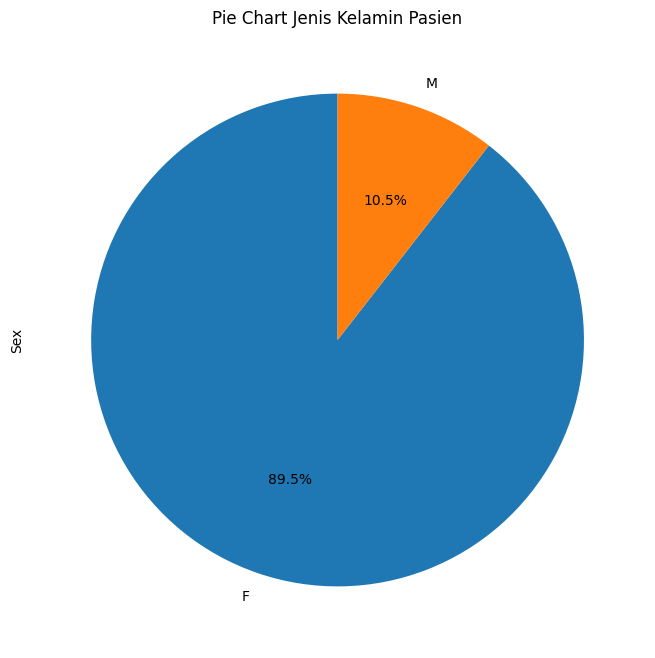
\includegraphics{sadam_files/figure-pdf/cell-9-output-1.png}

}

\end{figure}

\begin{Shaded}
\begin{Highlighting}[]

\NormalTok{plt.figure(figsize}\OperatorTok{=}\NormalTok{(}\DecValTok{10}\NormalTok{, }\DecValTok{6}\NormalTok{))}
\NormalTok{sns.histplot(df[}\StringTok{\textquotesingle{}Age\textquotesingle{}}\NormalTok{], bins}\OperatorTok{=}\DecValTok{30}\NormalTok{, kde}\OperatorTok{=}\VariableTok{True}\NormalTok{)}
\NormalTok{plt.title(}\StringTok{\textquotesingle{}Distribusi Umur Pasien\textquotesingle{}}\NormalTok{)}
\NormalTok{plt.xlabel(}\StringTok{\textquotesingle{}Umur\textquotesingle{}}\NormalTok{)}
\NormalTok{plt.ylabel(}\StringTok{\textquotesingle{}banyaknya pasien\textquotesingle{}}\NormalTok{)}
\NormalTok{plt.show()}

\NormalTok{plt.figure(figsize}\OperatorTok{=}\NormalTok{(}\DecValTok{10}\NormalTok{, }\DecValTok{6}\NormalTok{))}
\NormalTok{sns.boxplot(x}\OperatorTok{=}\StringTok{\textquotesingle{}Age\textquotesingle{}}\NormalTok{, y}\OperatorTok{=}\StringTok{\textquotesingle{}Status\textquotesingle{}}\NormalTok{, data}\OperatorTok{=}\NormalTok{df)}
\NormalTok{plt.title(}\StringTok{\textquotesingle{}Hubungan antara Umur dan Status Pasien\textquotesingle{}}\NormalTok{)}
\NormalTok{plt.xlabel(}\StringTok{\textquotesingle{}Status Pasien\textquotesingle{}}\NormalTok{)}
\NormalTok{plt.ylabel(}\StringTok{\textquotesingle{}Umur\textquotesingle{}}\NormalTok{)}
\NormalTok{plt.show()}
\end{Highlighting}
\end{Shaded}

\begin{figure}[H]

{\centering 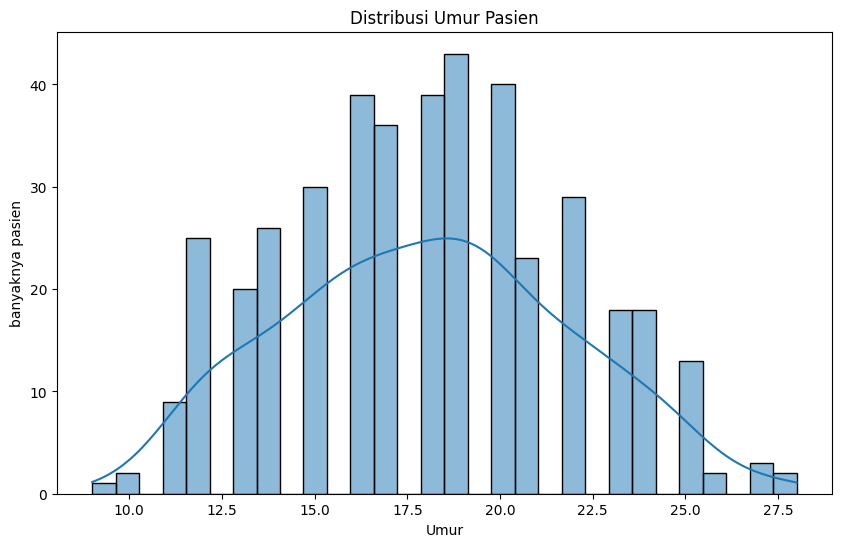
\includegraphics{sadam_files/figure-pdf/cell-10-output-1.png}

}

\end{figure}

\begin{figure}[H]

{\centering 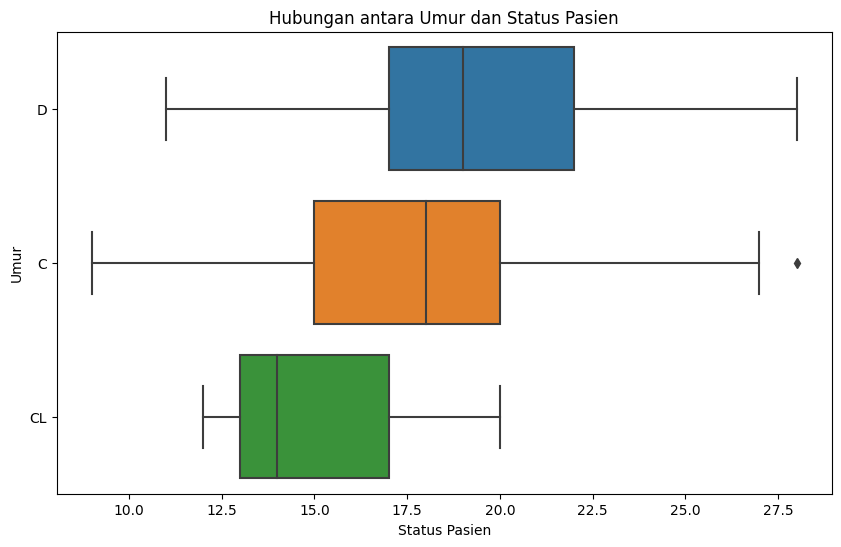
\includegraphics{sadam_files/figure-pdf/cell-10-output-2.png}

}

\end{figure}

\hypertarget{visual-tentang-seberapa-pengaruh-cirrhosis-patient-pada-umur-tertent-1}{%
\subsection{Visual tentang seberapa pengaruh Cirrhosis Patient pada umur
tertent}\label{visual-tentang-seberapa-pengaruh-cirrhosis-patient-pada-umur-tertent-1}}

\begin{enumerate}
\def\labelenumi{\arabic{enumi}.}
\item
  Rentang Usia Remaja (17-20 tahun): Pada rentang usia ini, terlihat
  adanya peningkatan signifikan dalam Cirrhosis Patient . Hal ini dapat
  menunjukkan bahwa remaja dalam kelompok usia ini mungkin memiliki
  faktor risiko tertentu yang berkontribusi pada prediksi penyakit hati.
  Status Pasien pada Usia 12-15 Tahun:
\item
  Prediksi status C (censored) yang lebih dominan pada kelompok usia
  12-15 tahun mungkin menunjukkan adanya kecenderungan untuk peristiwa
  yang tidak dapat diamati secara penuh. Ini bisa disebabkan oleh data
  yang tidak lengkap atau informasi yang tidak tersedia setelah periode
  pengamatan tertentu. Status Pasien pada Usia 14-20 Tahun:
\item
  Rentang usia 14-20 tahun menunjukkan kecenderungan prediksi status CL
  (censored karena transplantasi hati). Ini mungkin menandakan bahwa di
  dalam kelompok ini, pasien memiliki perawatan atau intervensi medis
  tertentu yang menyebabkan data pengamatan terhenti, seperti
  transplantasi hati. Status Pasien pada Usia 16-22 Tahun:
\item
  Pada usia ini, prediksi status D (kematian) mulai muncul lebih sering.
  Hal ini bisa menunjukkan tingkat keparahan penyakit atau faktor risiko
  tambahan yang dapat memengaruhi hasil pasien pada kelompok usia
  tersebut.
\end{enumerate}

Disini pada label mempunya 3 kelas yaitu: - C (Censored): Artinya pasien
tidak mengalami peristiwa akhir atau mati selama periode pengamatan.
Data pasien tersebut ``censored'' karena tidak ada informasi akhir yang
tersedia. - CL (Censored due to liver tx) Artinya pasien tidak mengalami
peristiwa akhir karena censored dan peristiwa censored tersebut terjadi
karena pasien menjalani transplantasi hati. - D (Death): Artinya pasien
mengalami kematian sebagai peristiwa akhir selama periode pengamatan

diatas bahwa data terbanyak yaitu categori C

Perbedaan C dan CL yaitu \textbf{C keterangannya tidak peristiwa akhir
atau mati tapi tidak melakukan transplantasi hati sedangkan CL juga
tidak ada tanda tanda peristiwa akhir tetapi harus menjalankan
transplantasi hati untuk menggantikan hati yang rusak}

\begin{Shaded}
\begin{Highlighting}[]
\NormalTok{jumlah\_kategori }\OperatorTok{=}\NormalTok{ df[}\StringTok{\textquotesingle{}Status\textquotesingle{}}\NormalTok{].nunique()}

\CommentTok{\# Menampilkan jumlah kategori}
\BuiltInTok{print}\NormalTok{(}\StringTok{"Jumlah kategori pada target:"}\NormalTok{, jumlah\_kategori)}
\end{Highlighting}
\end{Shaded}

\begin{verbatim}
Jumlah kategori pada target: 3
\end{verbatim}

Memisahkan antara fitur dengan label

\begin{Shaded}
\begin{Highlighting}[]
\NormalTok{X }\OperatorTok{=}\NormalTok{ df.drop([}\StringTok{\textquotesingle{}Status\textquotesingle{}}\NormalTok{,}\StringTok{\textquotesingle{}ID\textquotesingle{}}\NormalTok{], axis}\OperatorTok{=}\DecValTok{1}\NormalTok{)}
\NormalTok{y }\OperatorTok{=}\NormalTok{ df[}\StringTok{"Status"}\NormalTok{]}
\end{Highlighting}
\end{Shaded}

\hypertarget{seleksi-fitur-1}{%
\section{Seleksi fitur}\label{seleksi-fitur-1}}

sebelum melakukan preprocessing data alangkah baiknya untuk
menyeleksikan fitur fitur yang menurut kita adalah fitur yang tidak
berpengaruh terhadap dataset dan mengurangi beban dataset agar tidak
menyebabkan overfitting

Disini saya menggunakan sckit learn untuk melakukan selection pada fitur
- yang pertama saya menentukan banyaknya fitur terdapat N = banyak
fitur, fitur yang ada didataset adalah 19 fitur - Jumlah fitur terbaik
yang terpilih disesuaikan dengan nilai K di atas - ambil data data pada
setiap fitur menggunakan funtion colomns dan nama pada fitur akan
dimasukan kedalam selected\_feature\_names - lalu proses melakukan
perhitungan statistik ANOVA dengan rumus

\[
F = \frac{MSB}{MSW}
\] MSB atau mean square antar kelompok (mean square between groups).
dapat dari rumus ini :

\[
MSB = \frac{\sum_{i=1}^{k} n_i (\bar{X}_i - \bar{X}_{\text{total}})^2}{k - 1}
\] dan MSW atau mean square dalam kelompok (mean square within groups)

\[
MSW = \frac{\sum_{i=1}^{k} \sum_{j=1}^{n_i} (X_{ij} - \bar{X}_i)^2}{N - k}
\] Untuk hasil akhirnya saya menghapus 8 fitur yang menurut saya tidak
akan berpengaruh terhadap dataset saya

\begin{Shaded}
\begin{Highlighting}[]
\CommentTok{\# Misalkan \textquotesingle{}Feature1\textquotesingle{} dan \textquotesingle{}Feature2\textquotesingle{} adalah nama dua fitur yang ingin diubah}
\NormalTok{X[}\StringTok{\textquotesingle{}Drug\textquotesingle{}}\NormalTok{] }\OperatorTok{=}\NormalTok{ X[}\StringTok{\textquotesingle{}Drug\textquotesingle{}}\NormalTok{].astype(}\StringTok{\textquotesingle{}category\textquotesingle{}}\NormalTok{).cat.codes}
\NormalTok{X[}\StringTok{\textquotesingle{}Ascites\textquotesingle{}}\NormalTok{] }\OperatorTok{=}\NormalTok{ X[}\StringTok{\textquotesingle{}Ascites\textquotesingle{}}\NormalTok{].astype(}\StringTok{\textquotesingle{}category\textquotesingle{}}\NormalTok{).cat.codes}
\NormalTok{X[}\StringTok{\textquotesingle{}Hepatomegaly\textquotesingle{}}\NormalTok{] }\OperatorTok{=}\NormalTok{ X[}\StringTok{\textquotesingle{}Hepatomegaly\textquotesingle{}}\NormalTok{].astype(}\StringTok{\textquotesingle{}category\textquotesingle{}}\NormalTok{).cat.codes}
\NormalTok{X[}\StringTok{\textquotesingle{}Spiders\textquotesingle{}}\NormalTok{] }\OperatorTok{=}\NormalTok{ X[}\StringTok{\textquotesingle{}Spiders\textquotesingle{}}\NormalTok{].astype(}\StringTok{\textquotesingle{}category\textquotesingle{}}\NormalTok{).cat.codes}
\NormalTok{X[}\StringTok{\textquotesingle{}Stage\textquotesingle{}}\NormalTok{] }\OperatorTok{=}\NormalTok{ X[}\StringTok{\textquotesingle{}Stage\textquotesingle{}}\NormalTok{].astype(}\StringTok{\textquotesingle{}category\textquotesingle{}}\NormalTok{).cat.codes}
\NormalTok{X[}\StringTok{\textquotesingle{}Sex\textquotesingle{}}\NormalTok{] }\OperatorTok{=}\NormalTok{ X[}\StringTok{\textquotesingle{}Sex\textquotesingle{}}\NormalTok{].astype(}\StringTok{\textquotesingle{}category\textquotesingle{}}\NormalTok{).cat.codes}
\NormalTok{X[}\StringTok{\textquotesingle{}Edema\textquotesingle{}}\NormalTok{] }\OperatorTok{=}\NormalTok{ X[}\StringTok{\textquotesingle{}Edema\textquotesingle{}}\NormalTok{].astype(}\StringTok{\textquotesingle{}category\textquotesingle{}}\NormalTok{).cat.codes}

\end{Highlighting}
\end{Shaded}

\begin{Shaded}
\begin{Highlighting}[]
\NormalTok{selector }\OperatorTok{=}\NormalTok{ SelectKBest(score\_func}\OperatorTok{=}\NormalTok{f\_classif, k}\OperatorTok{=}\DecValTok{18}\NormalTok{)  }\CommentTok{\# K adalah jumlah fitur terbaik yang akan dipilih}

\CommentTok{\# \# Lakukan seleksi fitur}
\NormalTok{selector.fit(X, y)}

\CommentTok{\# \# Tampilkan hasil seleksi fitur}
\CommentTok{\# \# Jumlah fitur terbaik yang terpilih disesuaikan dengan nilai K di atas}
\NormalTok{selected\_features }\OperatorTok{=}\NormalTok{ selector.get\_support(indices}\OperatorTok{=}\VariableTok{True}\NormalTok{)}

\CommentTok{\# \# Ambil nama{-}nama fitur yang dipilih}
\CommentTok{\# selected\_feature\_names = [data.feature\_names[i] for i in selected\_features]}

\CommentTok{\# \# Hitung skor statistik untuk setiap fitur}
\CommentTok{\# scores = selector.scores\_[selected\_features]}

\NormalTok{feature\_names }\OperatorTok{=}\NormalTok{ X.columns}

\CommentTok{\# Pilih nama{-}nama fitur yang dipilih}
\NormalTok{selected\_feature\_names }\OperatorTok{=}\NormalTok{ [feature\_names[i] }\ControlFlowTok{for}\NormalTok{ i }\KeywordTok{in}\NormalTok{ selected\_features]}

\CommentTok{\# Sisa kode Anda tetap sama}
\CommentTok{\# Hitung skor statistik untuk setiap fitur}
\NormalTok{scores }\OperatorTok{=}\NormalTok{ selector.scores\_[selected\_features]}


\CommentTok{\# Membuat bar chart}
\NormalTok{plt.figure(figsize}\OperatorTok{=}\NormalTok{(}\DecValTok{10}\NormalTok{, }\DecValTok{6}\NormalTok{))}
\NormalTok{plt.bar(selected\_feature\_names, scores, color}\OperatorTok{=}\StringTok{\textquotesingle{}skyblue\textquotesingle{}}\NormalTok{)}
\NormalTok{plt.xlabel(}\StringTok{\textquotesingle{}Fitur\textquotesingle{}}\NormalTok{)}
\NormalTok{plt.ylabel(}\StringTok{\textquotesingle{}Skor Statistik\textquotesingle{}}\NormalTok{)}
\NormalTok{plt.title(}\StringTok{\textquotesingle{}Skor Statistik untuk Fitur{-}Fitur Terpilih\textquotesingle{}}\NormalTok{)}
\NormalTok{plt.xticks(rotation}\OperatorTok{=}\DecValTok{45}\NormalTok{)}
\NormalTok{plt.tight\_layout()}

\CommentTok{\# Menampilkan grafik}
\NormalTok{plt.show()}
\end{Highlighting}
\end{Shaded}

\begin{figure}[H]

{\centering 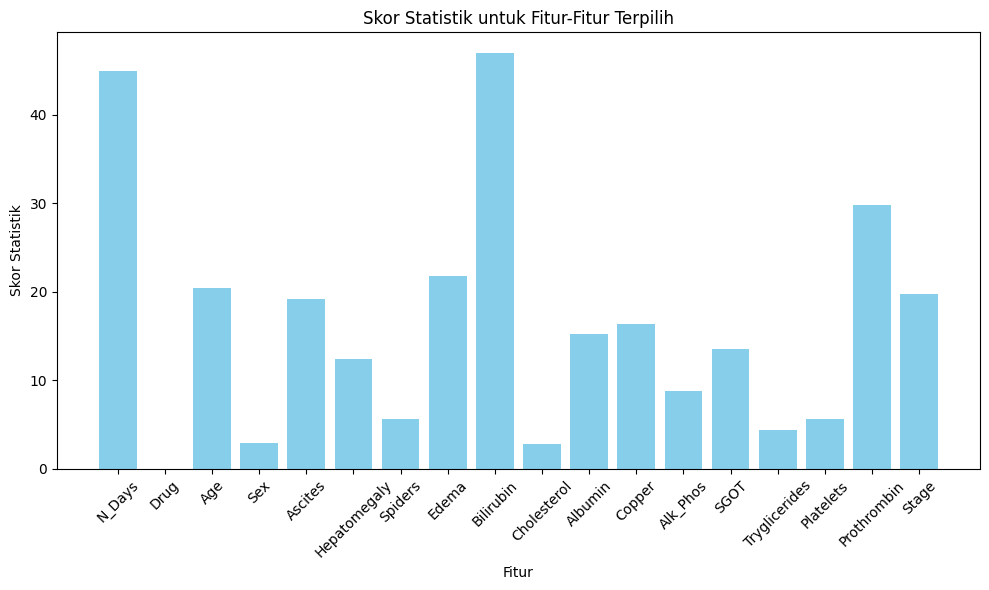
\includegraphics{sadam_files/figure-pdf/cell-14-output-1.png}

}

\end{figure}

\begin{Shaded}
\begin{Highlighting}[]
\NormalTok{X }\OperatorTok{=}\NormalTok{ df.drop([}\StringTok{\textquotesingle{}N\_Days\textquotesingle{}}\NormalTok{,}\StringTok{\textquotesingle{}ID\textquotesingle{}}\NormalTok{,}\StringTok{\textquotesingle{}Status\textquotesingle{}}\NormalTok{,}\StringTok{\textquotesingle{}Drug\textquotesingle{}}\NormalTok{,}\StringTok{\textquotesingle{}Sex\textquotesingle{}}\NormalTok{,}\StringTok{\textquotesingle{}Spiders\textquotesingle{}}\NormalTok{,}\StringTok{\textquotesingle{}Cholesterol\textquotesingle{}}\NormalTok{,}\StringTok{\textquotesingle{}Tryglicerides\textquotesingle{}}\NormalTok{,}\StringTok{\textquotesingle{}Platelets\textquotesingle{}}\NormalTok{], axis}\OperatorTok{=}\DecValTok{1}\NormalTok{)}
\NormalTok{X}
\end{Highlighting}
\end{Shaded}

\begin{longtable}[]{@{}llllllllllll@{}}
\toprule\noalign{}
& Age & Ascites & Hepatomegaly & Edema & Bilirubin & Albumin & Copper &
Alk\_Phos & SGOT & Prothrombin & Stage \\
\midrule\noalign{}
\endhead
\bottomrule\noalign{}
\endlastfoot
0 & 21 & Y & Y & Y & 14.5 & 2.60 & 156.0 & 1718.0 & 137.95 & 12.2 &
4.0 \\
1 & 20 & N & Y & N & 1.1 & 4.14 & 54.0 & 7394.8 & 113.52 & 10.6 & 3.0 \\
2 & 25 & N & N & S & 1.4 & 3.48 & 210.0 & 516.0 & 96.10 & 12.0 & 4.0 \\
3 & 19 & N & Y & S & 1.8 & 2.54 & 64.0 & 6121.8 & 60.63 & 10.3 & 4.0 \\
4 & 13 & N & Y & N & 3.4 & 3.53 & 143.0 & 671.0 & 113.15 & 10.9 & 3.0 \\
... & ... & ... & ... & ... & ... & ... & ... & ... & ... & ... & ... \\
413 & 24 & N & Y & N & 1.2 & 2.96 & 186.0 & 2115.0 & 136.00 & 10.9 &
3.0 \\
414 & 14 & N & Y & N & 0.9 & 3.83 & 186.0 & 2115.0 & 136.00 & 11.2 &
4.0 \\
415 & 20 & N & Y & N & 1.6 & 3.42 & 186.0 & 2115.0 & 136.00 & 9.9 &
3.0 \\
416 & 21 & N & Y & N & 0.8 & 3.75 & 186.0 & 2115.0 & 136.00 & 10.4 &
3.0 \\
417 & 19 & N & Y & N & 0.7 & 3.29 & 186.0 & 2115.0 & 136.00 & 10.6 &
4.0 \\
\end{longtable}

\hypertarget{mengganti-categori-menjadi-numerik-1}{%
\section{Mengganti categori menjadi
numerik}\label{mengganti-categori-menjadi-numerik-1}}

Sebelum melakukan preprosessing pada dataset saya diketahui memiliki
categori yang harus diganti menjadi numerik, maka saya gunakan code
seperti dibawah :

\begin{Shaded}
\begin{Highlighting}[]

\NormalTok{X[}\StringTok{\textquotesingle{}Ascites\textquotesingle{}}\NormalTok{] }\OperatorTok{=}\NormalTok{ X[}\StringTok{\textquotesingle{}Ascites\textquotesingle{}}\NormalTok{].astype(}\StringTok{\textquotesingle{}category\textquotesingle{}}\NormalTok{).cat.codes}
\NormalTok{X[}\StringTok{\textquotesingle{}Hepatomegaly\textquotesingle{}}\NormalTok{] }\OperatorTok{=}\NormalTok{ X[}\StringTok{\textquotesingle{}Hepatomegaly\textquotesingle{}}\NormalTok{].astype(}\StringTok{\textquotesingle{}category\textquotesingle{}}\NormalTok{).cat.codes}
\NormalTok{X[}\StringTok{\textquotesingle{}Edema\textquotesingle{}}\NormalTok{] }\OperatorTok{=}\NormalTok{ X[}\StringTok{\textquotesingle{}Edema\textquotesingle{}}\NormalTok{].astype(}\StringTok{\textquotesingle{}category\textquotesingle{}}\NormalTok{).cat.codes}
\NormalTok{X}
\end{Highlighting}
\end{Shaded}

\begin{longtable}[]{@{}llllllllllll@{}}
\toprule\noalign{}
& Age & Ascites & Hepatomegaly & Edema & Bilirubin & Albumin & Copper &
Alk\_Phos & SGOT & Prothrombin & Stage \\
\midrule\noalign{}
\endhead
\bottomrule\noalign{}
\endlastfoot
0 & 21 & 1 & 1 & 2 & 14.5 & 2.60 & 156.0 & 1718.0 & 137.95 & 12.2 &
4.0 \\
1 & 20 & 0 & 1 & 0 & 1.1 & 4.14 & 54.0 & 7394.8 & 113.52 & 10.6 & 3.0 \\
2 & 25 & 0 & 0 & 1 & 1.4 & 3.48 & 210.0 & 516.0 & 96.10 & 12.0 & 4.0 \\
3 & 19 & 0 & 1 & 1 & 1.8 & 2.54 & 64.0 & 6121.8 & 60.63 & 10.3 & 4.0 \\
4 & 13 & 0 & 1 & 0 & 3.4 & 3.53 & 143.0 & 671.0 & 113.15 & 10.9 & 3.0 \\
... & ... & ... & ... & ... & ... & ... & ... & ... & ... & ... & ... \\
413 & 24 & 0 & 1 & 0 & 1.2 & 2.96 & 186.0 & 2115.0 & 136.00 & 10.9 &
3.0 \\
414 & 14 & 0 & 1 & 0 & 0.9 & 3.83 & 186.0 & 2115.0 & 136.00 & 11.2 &
4.0 \\
415 & 20 & 0 & 1 & 0 & 1.6 & 3.42 & 186.0 & 2115.0 & 136.00 & 9.9 &
3.0 \\
416 & 21 & 0 & 1 & 0 & 0.8 & 3.75 & 186.0 & 2115.0 & 136.00 & 10.4 &
3.0 \\
417 & 19 & 0 & 1 & 0 & 0.7 & 3.29 & 186.0 & 2115.0 & 136.00 & 10.6 &
4.0 \\
\end{longtable}

diatas terdapat cara untuk menggantikan sebuah type kategori menjadi
numerik, terdapat fungsi yang saya pakai :

\begin{itemize}
\item
  astype(`category') , funtion tersebut untuk memberi tahu bahwa pada
  fitur tersebut adalah type category
\item
  cat.codes untuk mengubah category menjadi numerik, Bilangan bulat yang
  diberikan dimulai dari 0 dan terus bertambah seiring dengan munculnya
  nilai kategori yang baru. contohnya pada fitur Sex mempunyai 2
  category yaitu wanita dan lelaki, maka wanita akan diganti menjadi 0
  dan lelaki akan menjadi 1
\end{itemize}

\begin{Shaded}
\begin{Highlighting}[]

\ImportTok{from}\NormalTok{ sklearn.preprocessing }\ImportTok{import}\NormalTok{ MinMaxScaler}
\end{Highlighting}
\end{Shaded}

\bookmarksetup{startatroot}

\hypertarget{preprocessing-data-1}{%
\chapter{Preprocessing data}\label{preprocessing-data-1}}

\hypertarget{split-data-menjadi-train-data-dan-test-data-1}{%
\section{Split data menjadi train data dan test
data}\label{split-data-menjadi-train-data-dan-test-data-1}}

train\_test\_split adalah suatu fungsi dalam library scikit-learn yang
digunakan untuk membagi dataset menjadi dua set, yaitu set pelatihan
(training set) dan set pengujian (testing set). Pemisahan ini bertujuan
untuk melakukan pelatihan model pada set pelatihan dan menguji kinerja
model pada set pengujian. Fungsi ini sangat umum digunakan dalam proses
machine learning untuk menghindari overfitting dan mengevaluasi
kemampuan generalisasi dari model yang telah dilatih

\begin{enumerate}
\def\labelenumi{\arabic{enumi}.}
\item
  test\_size (opsional): Menentukan ukuran set pengujian sebagai
  proporsi dari seluruh dataset. Nilai ini bisa berupa pecahan
  (misalnya, 0.2 untuk 20\%) atau bilangan bulat yang menyatakan jumlah
  sampel yang akan ditempatkan di set pengujian.
\item
  random\_state (opsional): Digunakan untuk mengontrol randomization
  selama pembagian dataset. Jika nilai ini diberikan, pemisahan dataset
  akan tetap konsisten setiap kali fungsi ini dijalankan
\end{enumerate}

\begin{Shaded}
\begin{Highlighting}[]
\NormalTok{X\_train, X\_test, y\_train, y\_test }\OperatorTok{=}\NormalTok{ train\_test\_split(X, y, test\_size}\OperatorTok{=}\FloatTok{0.2}\NormalTok{, random\_state}\OperatorTok{=}\DecValTok{42}\NormalTok{)}
\end{Highlighting}
\end{Shaded}

\hypertarget{normalisasi-data-1}{%
\section{Normalisasi data}\label{normalisasi-data-1}}

Setelah melakukan understanding data maka melakukan preprocessing yang
dimana data akan di jadikan antara 0 sampai 1

dengan menggunakan minmaxScaller untuk menormalisasi data , dan
menggunakan train\_test\_split untuk mendapatkan data training dan data
testing

rumus MinmaxScaler:

\[
\text{Scaled Value} = \frac{\text{Original Value} - \text{Min}}{\text{Max} - \text{Min}}
\] - Original Value adalah nilai asli dari fitur.

\begin{itemize}
\item
  Min adalah nilai minimum dari fitur.
\item
  Max adalah nilai maksimum dari fitur.
\end{itemize}

\begin{enumerate}
\def\labelenumi{\arabic{enumi}.}
\item
  fit\_transform Fungsinya ini menghitung parameter normalisasi dari
  dataset (seperti nilai minimum dan maksimum) dan kemudian
  mengaplikasikan normalisasi pada dataset tersebut. Fungsi ini berguna
  untuk menghitung parameter normalisasi berdasarkan data pelatihan dan
  sekaligus menerapkan normalisasi tersebut.
\item
  Setelah kita telah menggunakan fit\_transform pada data pelatihan,
  kita dapat menggunakan metode transform pada data pengujian (dan data
  lainnya yang ingin dinormalisasi) menggunakan parameter normalisasi
  yang telah dihitung sebelumnya. Metode ini hanya melakukan normalisasi
  tanpa perlu menghitung parameter normalisasi lagi.
\end{enumerate}

\begin{Shaded}
\begin{Highlighting}[]
\NormalTok{scaler }\OperatorTok{=}\NormalTok{ MinMaxScaler()}
\NormalTok{X\_train\_scaler }\OperatorTok{=}\NormalTok{ scaler.fit\_transform(X\_train)}
\NormalTok{X\_test\_scaler }\OperatorTok{=}\NormalTok{ scaler.transform(X\_test)}
\NormalTok{x }\OperatorTok{=}\NormalTok{ pd.DataFrame(X\_train,columns}\OperatorTok{=}\NormalTok{X.columns)}
\NormalTok{x}
\end{Highlighting}
\end{Shaded}

\begin{longtable}[]{@{}llllllllllll@{}}
\toprule\noalign{}
& Age & Ascites & Hepatomegaly & Edema & Bilirubin & Albumin & Copper &
Alk\_Phos & SGOT & Prothrombin & Stage \\
\midrule\noalign{}
\endhead
\bottomrule\noalign{}
\endlastfoot
336 & 20 & 0 & 1 & 0 & 1.8 & 3.64 & 186.0 & 2115.0 & 136.00 & 10.0 &
3.0 \\
31 & 19 & 0 & 1 & 0 & 1.8 & 3.34 & 101.0 & 7277.0 & 82.56 & 10.6 &
4.0 \\
84 & 17 & 0 & 1 & 0 & 2.1 & 3.48 & 58.0 & 2045.0 & 89.90 & 11.5 & 4.0 \\
287 & 17 & 0 & 1 & 1 & 8.7 & 3.89 & 107.0 & 637.0 & 117.00 & 9.6 &
2.0 \\
317 & 15 & 0 & 1 & 0 & 0.7 & 3.68 & 186.0 & 2115.0 & 136.00 & 9.5 &
2.0 \\
... & ... & ... & ... & ... & ... & ... & ... & ... & ... & ... & ... \\
71 & 11 & 0 & 0 & 0 & 0.5 & 3.54 & 51.0 & 1243.0 & 122.45 & 10.0 &
3.0 \\
106 & 22 & 0 & 0 & 0 & 0.6 & 4.03 & 10.0 & 648.0 & 71.30 & 17.1 & 1.0 \\
270 & 18 & 0 & 1 & 0 & 1.0 & 3.50 & 94.0 & 955.0 & 111.00 & 9.7 & 3.0 \\
348 & 19 & 0 & 1 & 0 & 1.4 & 3.82 & 186.0 & 2115.0 & 136.00 & 10.3 &
2.0 \\
102 & 17 & 1 & 1 & 2 & 2.5 & 3.67 & 57.0 & 1273.0 & 119.35 & 11.1 &
4.0 \\
\end{longtable}

\bookmarksetup{startatroot}

\hypertarget{modeling-data-1}{%
\chapter{Modeling data}\label{modeling-data-1}}

\hypertarget{melatih-model-menggunakan-decision-tree-1}{%
\section{Melatih Model menggunakan decision
tree}\label{melatih-model-menggunakan-decision-tree-1}}

Decision tree (pohon keputusan) adalah model prediktif yang digunakan
dalam machine learning dan data mining. Model ini mengambil bentuk pohon
dengan setiap simpul (node) yang mewakili keputusan atau pengujian
terhadap suatu fitur, cabang (branch) yang mengarah ke simpul lainnya,
dan daun (leaf) yang memberikan hasil atau prediksi. Decision tree
digunakan untuk tugas klasifikasi dan regresi.

\begin{equation}
\text{Jika } X_i \leq T \text{ maka cabang kiri, else cabang kanan}
\end{equation}

\begin{Shaded}
\begin{Highlighting}[]
\NormalTok{decision\_tree\_model }\OperatorTok{=}\NormalTok{ DecisionTreeClassifier()}
\CommentTok{\# Latih model}
\NormalTok{decision\_tree\_model.fit(X\_train, y\_train)}
\CommentTok{\# Prediksi dengan model}
\NormalTok{decision\_tree\_predictions }\OperatorTok{=}\NormalTok{ decision\_tree\_model.predict(X\_test)}
\CommentTok{\# Evaluasi kinerja model}
\NormalTok{decision\_tree\_accuracy }\OperatorTok{=}\NormalTok{ accuracy\_score(y\_test, decision\_tree\_predictions)}
\end{Highlighting}
\end{Shaded}

\hypertarget{melatih-model-menggunakan-random-forest-1}{%
\section{Melatih Model menggunakan Random
Forest}\label{melatih-model-menggunakan-random-forest-1}}

Random Forest adalah sebuah algoritma machine learning yang digunakan
untuk tugas klasifikasi, regresi, dan pengurangan dimensi. Ini merupakan
jenis algoritma ensemble, yang menggabungkan beberapa model untuk
meningkatkan kinerja dan kestabilan prediksi. Algoritma Random Forest
membangun beberapa pohon keputusan selama pelatihan dan menggabungkan
hasil prediksi dari pohon-pohon tersebut untuk membuat prediksi yang
lebih akurat dan stabil

\begin{enumerate}
\def\labelenumi{\arabic{enumi}.}
\item
  Prediksi pada Pohon Keputusan \[
  \text{Prediction}_{\text{tree}} = \text{MajorityClass}(\text{Samples in Leaf})
  \]
\item
  Aggregasi Prediksi dari Semua Pohon (Klasifikasi) \[
  \text{Final Prediction}_{\text{RF}} = \text{MajorityClass}(\text{Predictions from all Trees})
  \]
\item
  Aggregasi Prediksi dari Semua Pohon (Regresi) \[
  \text{Final Prediction}_{\text{RF}} = \text{Average}(\text{Predictions from all Trees})
  \]
\end{enumerate}

\begin{Shaded}
\begin{Highlighting}[]

\CommentTok{\# Buat model Random Forest}
\NormalTok{random\_forest\_model }\OperatorTok{=}\NormalTok{ RandomForestClassifier(n\_estimators}\OperatorTok{=}\DecValTok{100}\NormalTok{)}
\CommentTok{\# Latih model}
\NormalTok{random\_forest\_model.fit(X\_train, y\_train)}
\CommentTok{\# Prediksi dengan model}
\NormalTok{random\_forest\_predictions }\OperatorTok{=}\NormalTok{ random\_forest\_model.predict(X\_test)}
\CommentTok{\# Evaluasi kinerja model}
\NormalTok{random\_forest\_accuracy }\OperatorTok{=}\NormalTok{ accuracy\_score(y\_test, random\_forest\_predictions)}
\end{Highlighting}
\end{Shaded}

\hypertarget{melatih-model-menggunakan-logistic-regression}{%
\section{Melatih Model menggunakan Logistic
Regression}\label{melatih-model-menggunakan-logistic-regression}}

Logistic Regression (Regresi Logistik) adalah algoritma machine learning
yang digunakan untuk tugas klasifikasi. Meskipun memiliki kata
``regresi'' dalam namanya, logistic regression sebenarnya digunakan
untuk masalah klasifikasi biner, di mana tujuannya adalah memprediksi
kelas target yang memiliki dua kemungkinan nilai (biasanya 0 atau 1).

\[
P(Y=1) = \frac{1}{1 + e^{-(\beta_0 + \beta_1 X_1 + \beta_2 X_2 + \ldots + \beta_n X_n)}}
\]

\begin{itemize}
\tightlist
\item
  P(Y=1) adalah probabilitas kejadian
\item
  Y sama dengan 1.
\item
  e adalah basis logaritma natural.
\item
  b adalah bobot .
\item
  X adalah data .
\end{itemize}

\begin{Shaded}
\begin{Highlighting}[]
\NormalTok{model }\OperatorTok{=}\NormalTok{ LogisticRegression()}

\CommentTok{\# Latih model}
\NormalTok{model.fit(X\_train\_scaler, y\_train)}

\CommentTok{\# Prediksi dengan model}
\NormalTok{logistic\_regression\_predictions }\OperatorTok{=}\NormalTok{ model.predict(X\_test)}

\CommentTok{\# Evaluasi kinerja model}
\NormalTok{logistic\_regression\_accuracy }\OperatorTok{=}\NormalTok{ accuracy\_score(y\_test, logistic\_regression\_predictions)}
\end{Highlighting}
\end{Shaded}

\begin{verbatim}
/usr/local/lib/python3.10/dist-packages/sklearn/base.py:432: UserWarning: X has feature names, but LogisticRegression was fitted without feature names
  warnings.warn(
\end{verbatim}

\hypertarget{melatih-data-menggunakan-jaringan-saraf-tiruan-1}{%
\section{Melatih data menggunakan Jaringan Saraf
Tiruan}\label{melatih-data-menggunakan-jaringan-saraf-tiruan-1}}

Jaringan Saraf Tiruan (JST) atau Neural Networks adalah bagian integral
dari machine learning. Neural networks terinspirasi oleh struktur dan
fungsi otak manusia dan dapat digunakan untuk menangani tugas-tugas
kompleks seperti klasifikasi, regresi, pengenalan pola, dan bahkan
pembelajaran tugas-tugas yang lebih kompleks

\begin{Shaded}
\begin{Highlighting}[]

\CommentTok{\# Buat model Jaringan Saraf Tiruan}
\NormalTok{neural\_network\_model }\OperatorTok{=}\NormalTok{ MLPClassifier(hidden\_layer\_sizes}\OperatorTok{=}\NormalTok{(}\DecValTok{64}\NormalTok{, }\DecValTok{32}\NormalTok{), max\_iter}\OperatorTok{=}\DecValTok{1000}\NormalTok{, random\_state}\OperatorTok{=}\DecValTok{42}\NormalTok{)}

\CommentTok{\# Latih model}
\NormalTok{neural\_network\_model.fit(X\_train\_scaler, y\_train)}

\CommentTok{\# Prediksi dengan model}
\NormalTok{neural\_network\_predictions }\OperatorTok{=}\NormalTok{ neural\_network\_model.predict(X\_test)}

\CommentTok{\# Evaluasi kinerja model}
\NormalTok{neural\_network\_accuracy }\OperatorTok{=}\NormalTok{ accuracy\_score(y\_test, neural\_network\_predictions)}
\end{Highlighting}
\end{Shaded}

\begin{verbatim}
/usr/local/lib/python3.10/dist-packages/sklearn/neural_network/_multilayer_perceptron.py:686: ConvergenceWarning: Stochastic Optimizer: Maximum iterations (1000) reached and the optimization hasn't converged yet.
  warnings.warn(
/usr/local/lib/python3.10/dist-packages/sklearn/base.py:432: UserWarning: X has feature names, but MLPClassifier was fitted without feature names
  warnings.warn(
\end{verbatim}

\hypertarget{melatih-data-menggunakan-percepton-1}{%
\section{Melatih data menggunakan
Percepton}\label{melatih-data-menggunakan-percepton-1}}

Perceptron adalah model dasar dalam machine learning yang digunakan
untuk tugas klasifikasi biner. Perceptron dirancang untuk memodelkan
neuron dalam otak manusia dan dapat digunakan untuk memisahkan dua kelas
dengan menarik garis pemisah linier. Namun, perceptron memiliki
keterbatasan dan biasanya digunakan sebagai dasar untuk model neural
network yang lebih kompleks

\[
\text{Output} = \begin{cases}
1 & \text{jika } \sum_{i=1}^{n} w_i x_i + b > 0 \\
0 & \text{lainnya}
\end{cases}
\]

\begin{Shaded}
\begin{Highlighting}[]

\CommentTok{\# Buat model Perceptron}
\NormalTok{perceptron\_model }\OperatorTok{=}\NormalTok{ Perceptron(max\_iter}\OperatorTok{=}\DecValTok{1000}\NormalTok{, random\_state}\OperatorTok{=}\DecValTok{42}\NormalTok{)}

\CommentTok{\# Latih model Perceptron}
\NormalTok{perceptron\_model.fit(X\_train\_scaler, y\_train)}

\CommentTok{\# Prediksi dengan model Perceptron}
\NormalTok{perceptron\_predictions }\OperatorTok{=}\NormalTok{ perceptron\_model.predict(X\_test)}

\CommentTok{\# Evaluasi kinerja model Perceptron}
\NormalTok{perceptron\_accuracy }\OperatorTok{=}\NormalTok{ accuracy\_score(y\_test, perceptron\_predictions)}
\end{Highlighting}
\end{Shaded}

\begin{verbatim}
/usr/local/lib/python3.10/dist-packages/sklearn/base.py:432: UserWarning: X has feature names, but Perceptron was fitted without feature names
  warnings.warn(
\end{verbatim}

\bookmarksetup{startatroot}

\hypertarget{evaluasi-1}{%
\chapter{Evaluasi}\label{evaluasi-1}}

\begin{Shaded}
\begin{Highlighting}[]
\BuiltInTok{print}\NormalTok{(}\StringTok{"Akurasi decision\_tree:"}\NormalTok{, decision\_tree\_accuracy)}
\BuiltInTok{print}\NormalTok{(}\StringTok{"Akurasi Random Forest:"}\NormalTok{, random\_forest\_accuracy)}
\BuiltInTok{print}\NormalTok{(}\StringTok{"Akurasi Regresi Logistik:"}\NormalTok{, logistic\_regression\_accuracy)}
\BuiltInTok{print}\NormalTok{(}\StringTok{"Akurasi neural\_network:"}\NormalTok{, neural\_network\_accuracy)}
\BuiltInTok{print}\NormalTok{(}\StringTok{"Akurasi Perceptron:"}\NormalTok{, perceptron\_accuracy)}
\end{Highlighting}
\end{Shaded}

\begin{verbatim}
Akurasi decision_tree: 0.7380952380952381
Akurasi Random Forest: 0.75
Akurasi Regresi Logistik: 0.42857142857142855
Akurasi neural_network: 0.42857142857142855
Akurasi Perceptron: 0.42857142857142855
\end{verbatim}

Pada akurasi ini adalah paling tinggi di model yang lain, maka saya
memilih metode random forest, alasan lainnya mengapa menggunakan Random
Forest Dengan mempertimbangkan akurasinya lebih tinggi dari pada model
yang lain , Random Forest juga dapat mengurangi risiko overfitting pada
data pelatihan

\begin{Shaded}
\begin{Highlighting}[]
\CommentTok{\# import pickle}

\CommentTok{\# \# Simpan model ke file}
\CommentTok{\# with open(\textquotesingle{}/content/drive/MyDrive/PSD/Tugas4/saved.pkl\textquotesingle{}, \textquotesingle{}wb\textquotesingle{}) as file:}
\CommentTok{\#     pickle.dump(random\_forest\_model, file)}
\end{Highlighting}
\end{Shaded}

\begin{Shaded}
\begin{Highlighting}[]

\ImportTok{import}\NormalTok{ joblib}
\CommentTok{\# from sklearn.externals import joblib}
\NormalTok{joblib.dump(random\_forest\_model, }\StringTok{\textquotesingle{}/content/drive/MyDrive/PSD/Tugas4/saved\_data.joblib\textquotesingle{}}\NormalTok{)}
\end{Highlighting}
\end{Shaded}

\begin{verbatim}
['/content/drive/MyDrive/PSD/Tugas4/saved_data.joblib']
\end{verbatim}

\begin{Shaded}
\begin{Highlighting}[]
\NormalTok{loaded\_model }\OperatorTok{=}\NormalTok{ joblib.load(}\StringTok{\textquotesingle{}/content/drive/MyDrive/PSD/Tugas4/saved\_data.joblib\textquotesingle{}}\NormalTok{)}


\NormalTok{new\_data }\OperatorTok{=}\NormalTok{ [}\DecValTok{20}\NormalTok{,}\DecValTok{0}\NormalTok{,}\DecValTok{1}\NormalTok{,}\DecValTok{0}\NormalTok{,}\FloatTok{1.8}\NormalTok{,}\FloatTok{3.64}\NormalTok{,}\FloatTok{186.0}\NormalTok{,}\FloatTok{2115.0}\NormalTok{,}\FloatTok{136.00}\NormalTok{,}\FloatTok{10.0}\NormalTok{,}\FloatTok{3.0}\NormalTok{]}
\NormalTok{prediction }\OperatorTok{=}\NormalTok{ loaded\_model.predict([new\_data])}
\BuiltInTok{print}\NormalTok{(prediction)}
\end{Highlighting}
\end{Shaded}

\begin{verbatim}
['D']
\end{verbatim}

\begin{verbatim}
/usr/local/lib/python3.10/dist-packages/sklearn/base.py:439: UserWarning: X does not have valid feature names, but RandomForestClassifier was fitted with feature names
  warnings.warn(
\end{verbatim}

\bookmarksetup{startatroot}

\hypertarget{references}{%
\chapter*{References}\label{references}}
\addcontentsline{toc}{chapter}{References}

\markboth{References}{References}

\hypertarget{refs}{}
\begin{CSLReferences}{0}{0}
\end{CSLReferences}



\backmatter
\printindex

\end{document}
